\documentclass[output=paper]{LSP/langsci}  
\author{Yasuo Kumagai\affiliation{National Institute for Japanese Language and Linguistics, NINJAL}} 
\title{Developing the {L}inguistic {A}tlas of {J}apan {D}atabase and advancing analysis of geographical distributions of dialects}
\abstract{The Linguistic Atlas of Japan (LAJ) was published from 1966 to 1974. A total of 285 items (mainly from the lexical field) and 2400 localities were surveyed. 
% abstract too long, therefore removing material (JN)
% Since its publication, various nationwide quantitative studies using multivariate analyses and quantitative techniques have been conducted on the LAJ, including on dialect areas, geographical diffusion of standard forms, and so on. However, the lack of digital data has restricted the methods used in these quantitative studies. For example, the nationwide quantitative studies were conducted at the prefecture level. 
In 1999, we started constructing the Linguistic Atlas of Japan Database (LAJDB) with the aim of preserving the original survey materials (540000 cards) and advancing various uses of the LAJ. To explore the potential of the LAJDB in advancing quantitative approaches to the LAJ, I made some preliminary observations at the locality level concerning, for example, (1) geographical distributions of the frequency of standard forms, multiple answers, and informants’ (speakers’) comments on standard forms; (2) geographical distributions of degrees of linguistic similarities among localities; and (3) network representation of the degrees of linguistic similarities. These nationwide “high resolution” patterns of 2400 localities showed clear patterns and structures. Comparing these patterns and structures with each other and with extra-linguistic features, such as the network of roads, enables us to examine their relations in detail. The former nationwide, prefecture-level quantitative studies using the LAJ could not achieve such examination. I present some of these preliminary results and discuss several implications for advancing quantitative analysis using the LAJ.
}
\rohead{\thechapter\hspace{0.5em}Developing the {L}inguistic {A}tlas of {J}apan {D}atabase}

\maketitle 
\begin{document}

\section{Introduction}
The \textit{Linguistic Atlas of Japan} (\textit{LAJ}), with six volumes \citep{kokuritsu_kokugo_kenkyujo_nlri_nihon_1966-1}, is the first nationwide Japanese linguistic atlas based on a linguistic geographical survey method. Published from 1966 to 1974, it is one of the basic research materials in Japanese dialectology. Many studies on Japanese dialects have utilized the LAJ—including studies based on an interpretation of each linguistic map, such as \citet{sato_chiikishakai_1986}, \citet{tokugawa_hogenchirigaku_1993}, and \citet{kobayashi_hogengakuteki_2004}, as well as quantitative studies based on an accumulation of maps, such as \citet{takada_kotoba_1969}, \citet{hondo_gendai_1980}, \citet{kasai_hyojun_1981}, \citet{ichii_hogen_1993}, and \citet{inoue_keiryoteki_2001}.

However, quantitative studies that use the LAJ have certain limitations. First, such studies, which used each survey point as a unit of calculation, were restricted to examination of small areas. Next, the nationwide studies were mainly based on prefecture-unit calculations. For example, nationwide geographical distributions of standard word forms in the LAJ have been one of the most analyzed subjects in quantitative studies using the LAJ (e.g., \citealt{inoue_keiryoteki_2001}), but such studies are based on prefecture-level calculations,\footnote{Japan has 47 prefectures.} mainly due to difficulties in generating LAJ data at the locality level (e.g., \citealt[485, 498]{hondo_gendai_1980}). In these studies, researchers prepared their data individually by reading the printed maps. It would have been very laborious to prepare data in such a manner, and it would have been difficult to achieve accuracy everywhere. The lack of digital data certainly restricted the methods of quantitative studies utilizing the LAJ.

We have been developing the Linguistic Atlas of Japan Database (LAJDB), aiming to preserve the original survey materials and advance the utilization of the LAJ. The LAJDB provides data from 2400 survey localities. Calculations at the locality level enable researchers to observe “high resolution” geographical distribution patterns (approximately 50 times the resolution of 47 prefectures). These “high resolution” patterns enable researchers, for example, to trace various diffusion routes that former studies could not detect. Compared with the former studies using the LAJ, studies using the LAJDB can compare such diffusion routes with extra-linguistic features, such as road networks, to examine the relation among them in detail. The LAJDB provides not only the geographical distribution data of word forms but also the original survey card images. This feature proves useful for advancing the utilization of the LAJ. In section 2, I provide an overview of the LAJ and LAJDB. In section 3, I describe some results of preliminary observations to elucidate the potential of the LAJDB. 

\section{LAJ and the LAJ Database (LAJDB)}

The survey for the LAJ was conducted from 1957 to 1965 by the National Language Research Institute (NLRI), which preceded the present National Institute for Japanese Language and Linguistics (NINJAL). A total of 285 questionnaire items \citep[105--118]{kokuritsu_kokugo_kenkyujo_nlri_nihon_1966}, mainly pertaining to the lexical field (nouns, verbs and adjectives), and 2400 localities\footnote{The number of surveyed localities was not equal for each item. The approximate numbers are as follows: Of 285 items, 128 items were surveyed at 2400 localities, 36 items at 2000 localities, 55 items at 1700 localities, 62 items at 1000 localities, and 4 items at 400 localities \citep[22, 41]{kokuritsu_kokugo_kenkyujo_nlri_nihon_1966}.} were surveyed by 65 fieldworkers through personal interviews. In principle, one male informant (speaker) born before 1903\footnote{“One inhabitant was interrogated of each 40,000 people, but since the survey chose only male informants born before 1903, and since we know that there were 4,800,000 males of that age in the whole of Japan (1960 figures), our survey actually reproduces the speech of one out of 2000 of that stratum of the population” \citep[41--42]{kokuritsu_kokugo_kenkyujo_nlri_nihon_1966}.} and born at the given location (or, at least, who spent time there without interruption from the age of 3 to 15) was chosen as informant.\footnote{In principle, those whose residence in the locality had been interrupted by absences longer than 36 months were avoided.} As far as possible, those representing the general trend of occupation in their locality were chosen. Here, we may note that approximately 80\% of all localities are agricultural communities \citep[22, 42]{kokuritsu_kokugo_kenkyujo_nlri_nihon_1966}. Consequently, for practical reasons, male informants were chosen at 2392 localities (99.7\%) and female informants were chosen at eight localities. Concerning informants, 97\% were born between 1879 and 1903. Moreover, 63\% of informants were engaged in agricultural work, 21\% in commerce, and the rest in five other occupation categories \citep[24--26, 42, 43]{kokuritsu_kokugo_kenkyujo_nlri_nihon_1966}. Almost all informants of the LAJ can be described as “NORMs,” that is, non-mobile, older, rural males \citep[29]{chambers_dialectology_1998}. It was reported that “on an average about 6 localities were surveyed in every 1000 square kilometers, or an average of about 12 kilometers separates each surveyed locality” \citep[41]{kokuritsu_kokugo_kenkyujo_nlri_nihon_1966}. The LAJ covers the whole of Japan, and the maximum geographic distance for a locality pair is approximately 2960 km. \figref{fig:1} provides an example of maps from the LAJ.

During the survey period of the LAJ, after completing the questionnaire, each informant’s answer was copied to a separate card by fieldworkers. These cards, which number approximately 540000 \citep[38, 43]{kokuritsu_kokugo_kenkyujo_nlri_nihon_1966} and represent the materials of each answer from each locality, were used as original survey materials while editing the LAJ. On these cards, we can see the original phonetic transcriptions by the fieldworkers, informants’ comments, fieldworkers’ and editors’ notes and so on, which were utilized in editing the maps. However, the published LAJ hardly provided any of this information for users.\footnote{The editors of the LAJ prepared the materials “Nihon gengo chizu shiryô,” which listed the varieties corresponding to every linguistic form presented in the LAJ and the comments of informants and fieldworkers \citep[32, 33]{kokuritsu_kokugo_kenkyujo_nlri_nihon_1966}. These materials were recorded from the original survey cards in handwritten form. They need further proofreading, and the list is partially incomplete. To use this material, it is necessary to check the original survey cards for confirmation. The editors planned to publish the comments and notes \citep[44]{kokuritsu_kokugo_kenkyujo_nlri_nihon_1966}, but this plan was not realized.}

\begin{figure}
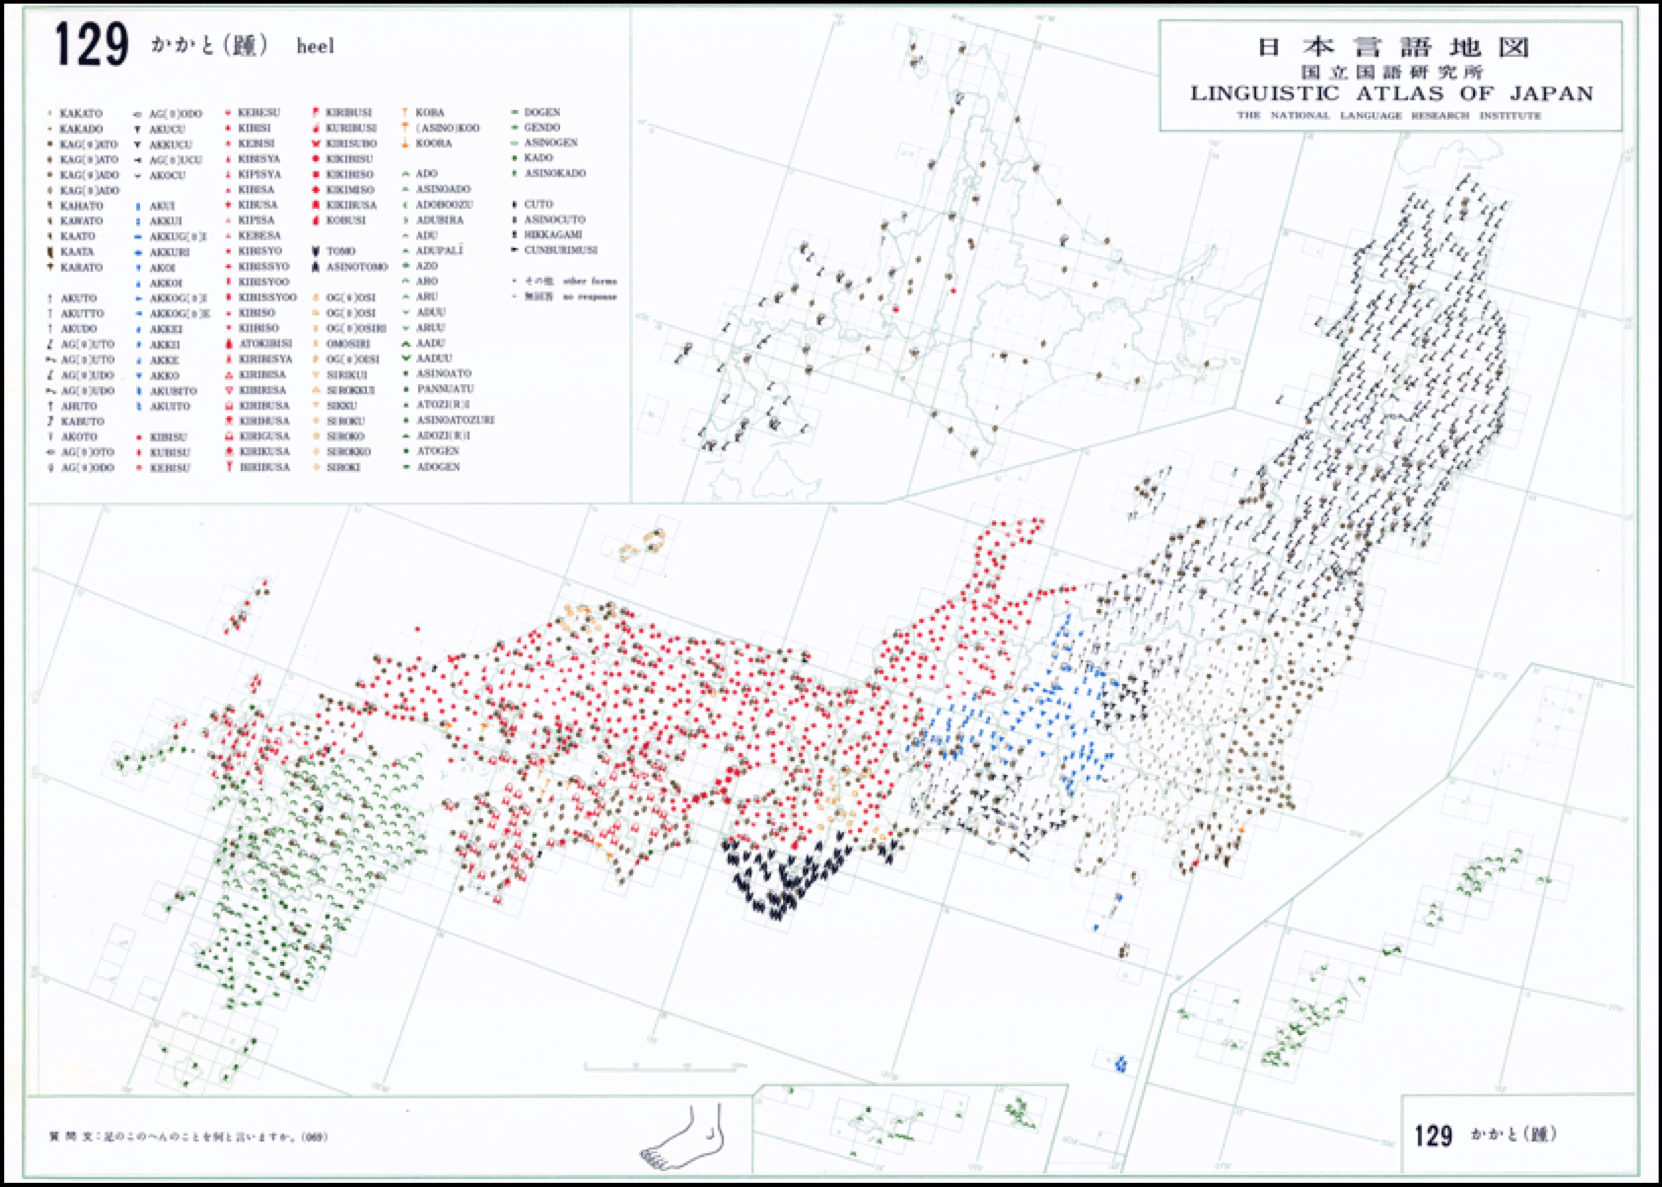
\includegraphics[width=0.8\textwidth]{illustrations/kuma_fig01}
\caption{A map from the LAJ (map 129: heel).}          
\label{fig:1}
\end{figure}  

\begin{figure}
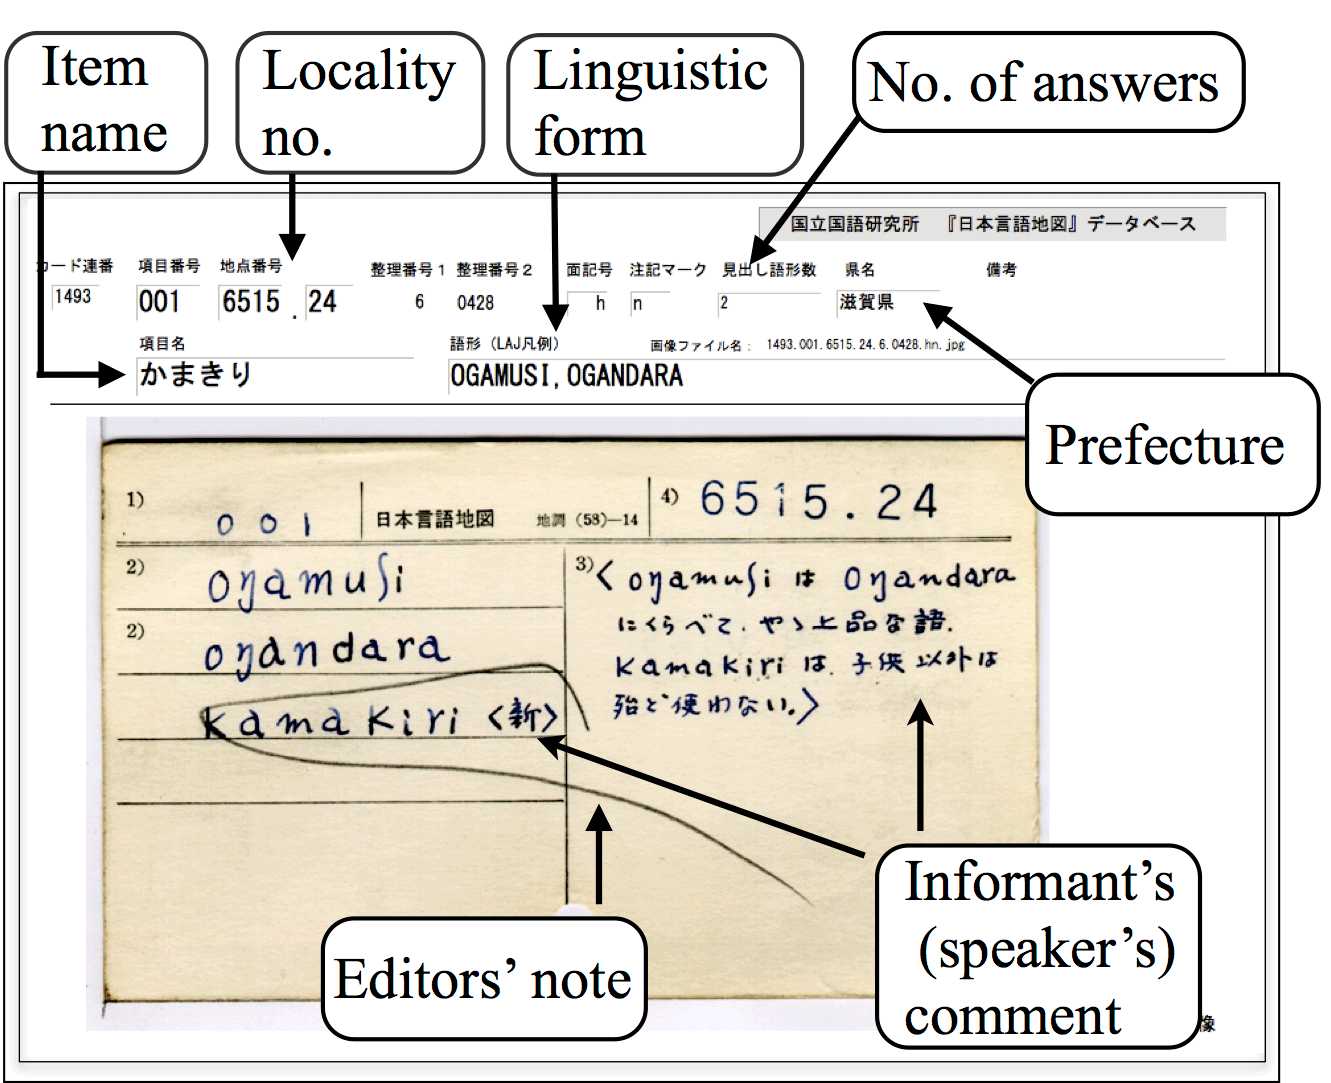
\includegraphics[width=0.8\textwidth]{illustrations/kuma_fig02}
\caption{A snapshot of the LAJDB image database.}        
\label{fig:2}
\end{figure} 

In 1999, with the aim of preserving these original survey materials and promoting the utilization of the LAJ, we began constructing the LAJDB (Kumagai 2013a, b).\footnote{ After the LAJ was published, the Grammar Atlas of Japan (GAJ, 6 volumes) was published between 1989 and 2006 by the NLRI (NLRI 1989–2006). Surveys were conducted from 1979 to 1982 in 807 localities. In the course of editing the GAJ, the use of computer in publishing the GAJ was developed and the GAJ data was made accessible to the public. However, in the days of the LAJ, computers were in the early stages of development and not available for publishing linguistic atlases.} The LAJDB comprises an image database of the original survey cards (\figref{fig:2}) and coded data corresponding to the published maps. The items of coded data include (a) locality number (systematically corresponding to degrees of longitude and latitude), (b) item name, (c) linguistic form on the legend of each map, (d) prefecture, (e) number of answers, (f) pattern of multiple answers, and so on. The original survey card images are linked to each entry of the coded data. While the linguistic forms shown on the maps from the LAJ are the result of the editor’s classifications of varieties recorded by the fieldworkers, the LAJ does not provide us with detailed information about the classifications. Combining the coded data from the LAJ and the original survey material card images, the LAJDB allows, for example, tracing of the classifications and interpretations completed by the editors. Moreover, the LAJDB facilitates close examination of the LAJ as a research material, reclassification of linguistic varieties based on other viewpoints, and utilization of informants’ comments and field workers’ and editors’ notes.

Currently, 119 items have been completed, corresponding to 43\% of the number of surveyed items (285 items) and 49\% of the number of items published as maps (240 items). The progress of the scanning of the original survey cards has reached approximately 90\% of the total number of items \citep[159]{kumagai_daikibo_2013}.

In addition, we have been preparing the following data for the LAJDB: (1) informant’s information provided in the LAJ \citep[47--102]{kokuritsu_kokugo_kenkyujo_nlri_nihon_1966}, such as (a) address (without house number), (b) year of birth, (c) occupation, (d) educational background (number of years), (e) absence from the locality (number of months), (f) experience of military service, (g) sex, (h) name of interviewer (fieldworker), (i) year of survey, and (j) questionnaire used; and (2) digital maps—in shapefile format, a standard file format for geographic information system (GIS) software—based on the “Introductory maps” from the LAJ compiled by the editors, including (a) basic maps from the LAJ, (b) topographical maps (showing mountain systems, river systems, etc.), (c) main roads in the Meiji period (approximately 1885), (d) the boundaries of the feudal domains during the Edo period (1664), and so on.

\section{Some preliminary observations from using the LAJDB}

\subsection{Dataset for preliminary observations}
As previously mentioned (see footnote 2), the number of surveyed localities for the LAJ was not equal for each item. Therefore, to explore the possibilities of the LAJDB, I selected 55 items from the LAJDB, in progress, with 2400 ± 1 survey points. We will call this dataset LAJDB55 data. The item numbers selected for LAJDB55 are as follows: (001), (005), 006, 007, (012), 032, 036, 038, 039, 048, 051, 052, (056), 057, 059, 060, 063, 064, 066, 067, 072, 076, 083, 089, 103, [104], [105], 110, 111, 116, 118, 119, (122), 124, (127), 129, 148, 149, (165), 174, 179, 185, (186), (187), (188), 191, 194, 200, 214, 215, (216), 219, 220, 221, and 223.

Furthermore, I created a subset—LAJDB42—of LAJDB55 to explore the distribution of the standard forms. In most cases, an item has one standard form; however, two or more forms were occasionally recognized as standard by the LAJ’s editors. In the above item numbers, those enclosed in parentheses are the ones in which two or more standard forms were recognized by the editors. No standard forms were explicitly stated for the items enclosed in square brackets []. For convenience in processing standard forms, I omitted the 13 items in  parentheses from LAJDB55 and acquired them from LAJDB42. Using the LAJDB55 and LAJDB42 datasets, I made some preliminary observations.

\subsection{Geographical frequency distributions of standard forms}
Leading studies using quantitative analysis of the LAJ have been performed by Fumio Inoue (\citealt{inoue_keiryoteki_2001}, etc.). \citet{inoue_keiryoteki_2001}, in a collection of his research of approximately 20 years, analyzed the usage rates of the standard forms of 84 LAJ items, summed up by prefecture (47 prefectures and Hachijô island, which belongs to Tokyo metropolitan area but whose dialect differs significantly from that of Tokyo). This data was originally prepared by Hisako Kasai (\citeyear{kasai_hyojun_1981}) by hand. Inoue input the data for quantitative analysis \citep[89]{inoue_keiryoteki_2001}. This data is known as the Kasai data. \citet{inoue_keiryoteki_2001} analyzed the Kasai data via multivariate analyses, quantitative techniques, and so on, in order to explore dialect areas, the geographical diffusion of dialects, the distribution of standard forms, and so on.

\figref{fig:3}\footnote{\figref{fig:3} was created based on Kasai’s (\citeyear{kasai_hyojun_1981}) calculation. Okinawa, located in the southernmost part of Japan, is not displayed in this figure due to space constraints.} shows the distribution of the usage rates of the standard forms of Kasai data on the map. With the Tokyo metropolitan area as the peak, the usage rate gradually declines toward the periphery, resembling a wave-like diffusion with Tokyo at its center. Hokkaido is an exception as it was a new settlement with people from mainland Japan.

It should be noted that the gridlines of the map are drawn based on the locality number system of the LAJ. The locality number system was based on topographical maps with a scale of 1:50000. Each block in the grid corresponds to 100 topographical maps of a 1:50000 scale. The size of each block in the grid is 2°30' east–west, 1°40' north–south. The gridlines that appear hereafter are similar.

\figref{fig:4} shows the usage rates of the standard forms according to LAJDB42 data based on the same calculation method as Kasai data, which shows similar distribution of Kasai data. In \figref{fig:5}, the usage rates of the standard forms of Kasai and LAJDB42 data are plotted in the descending order of the values of Kasai data for comparison. \figref{fig:5} indicates that Kasai data and LAJDB42 data show a very similar pattern overall. \figref{fig:6} shows the geographical distributions of the frequency (GDF) of the standard forms of LAJDB42 data by 2400 survey points. The GDF of standard forms was calculated by simply totaling the number of standard forms at each locality in the dataset. Patterns can be observed in detail, which could not be obtained from the prefecture-unit calculations of former studies. These “high resolution” patterns obtained using the LAJDB enable us to observe the diffusion routes more precisely. Comparing these distributions with the road networks, which play an important role in dialect diffusion, reveals interesting relationships. 

\begin{figure}
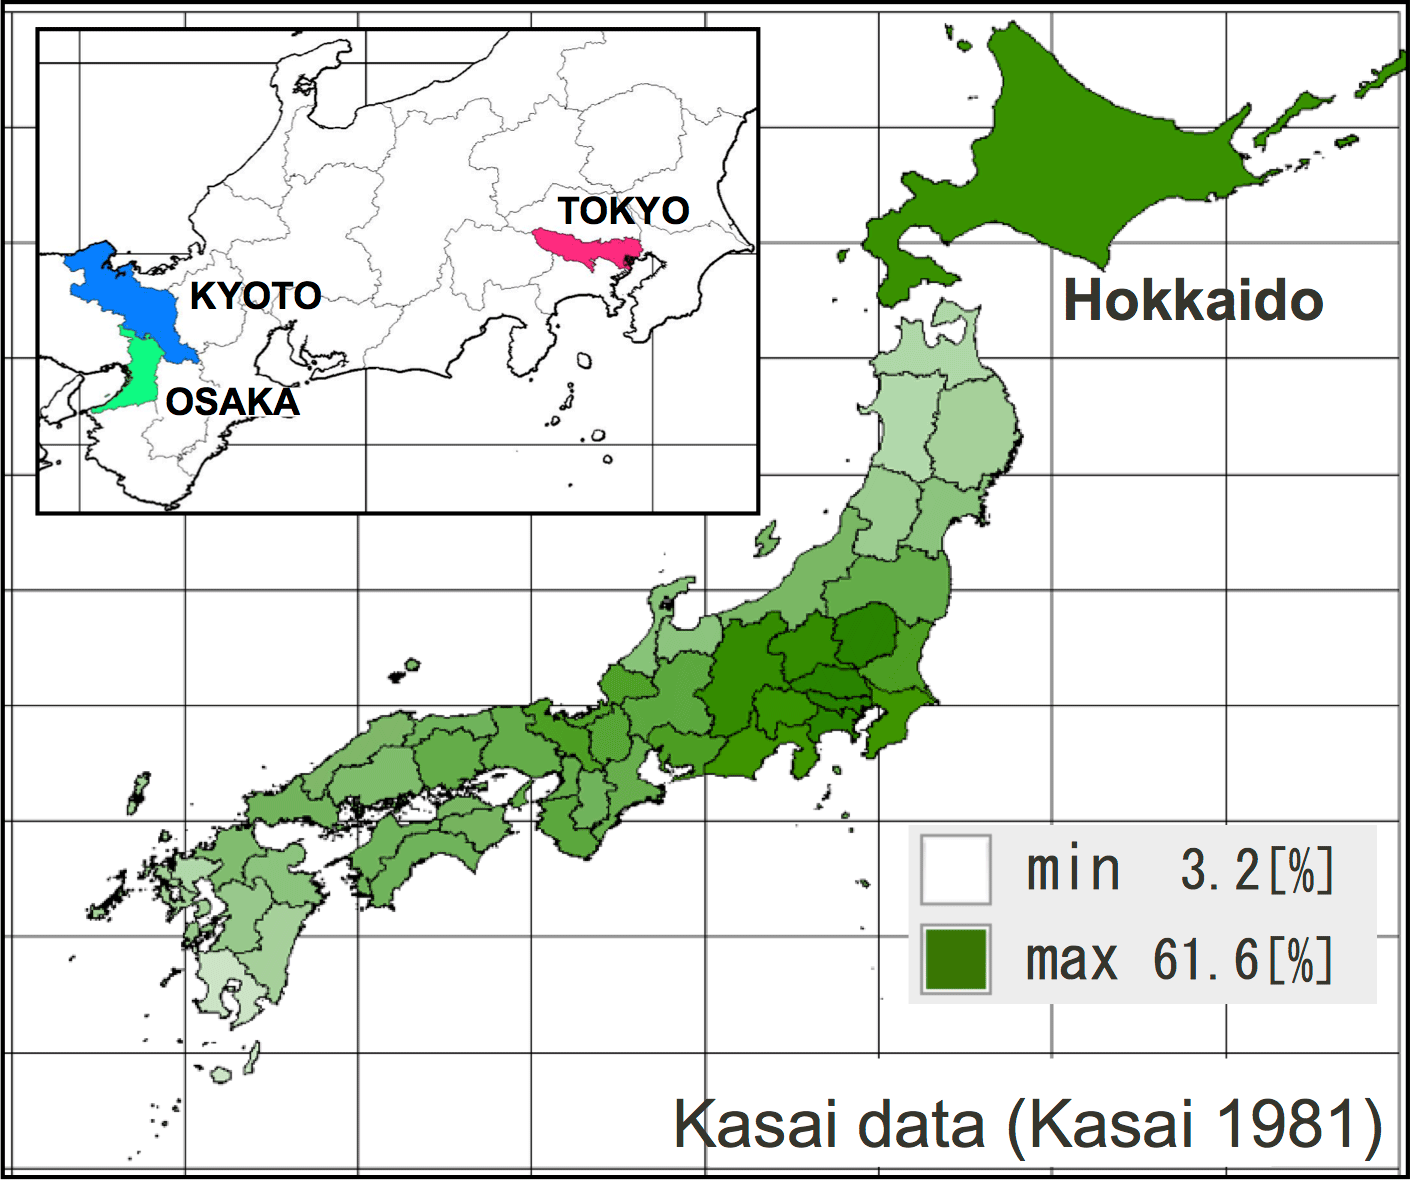
\includegraphics[width=0.8\textwidth]{illustrations/kuma_fig03}
\caption{Usage rates of standard forms of 84 LAJ items, summed up by prefecture.}          
\label{fig:3}
\end{figure} 
\begin{figure}
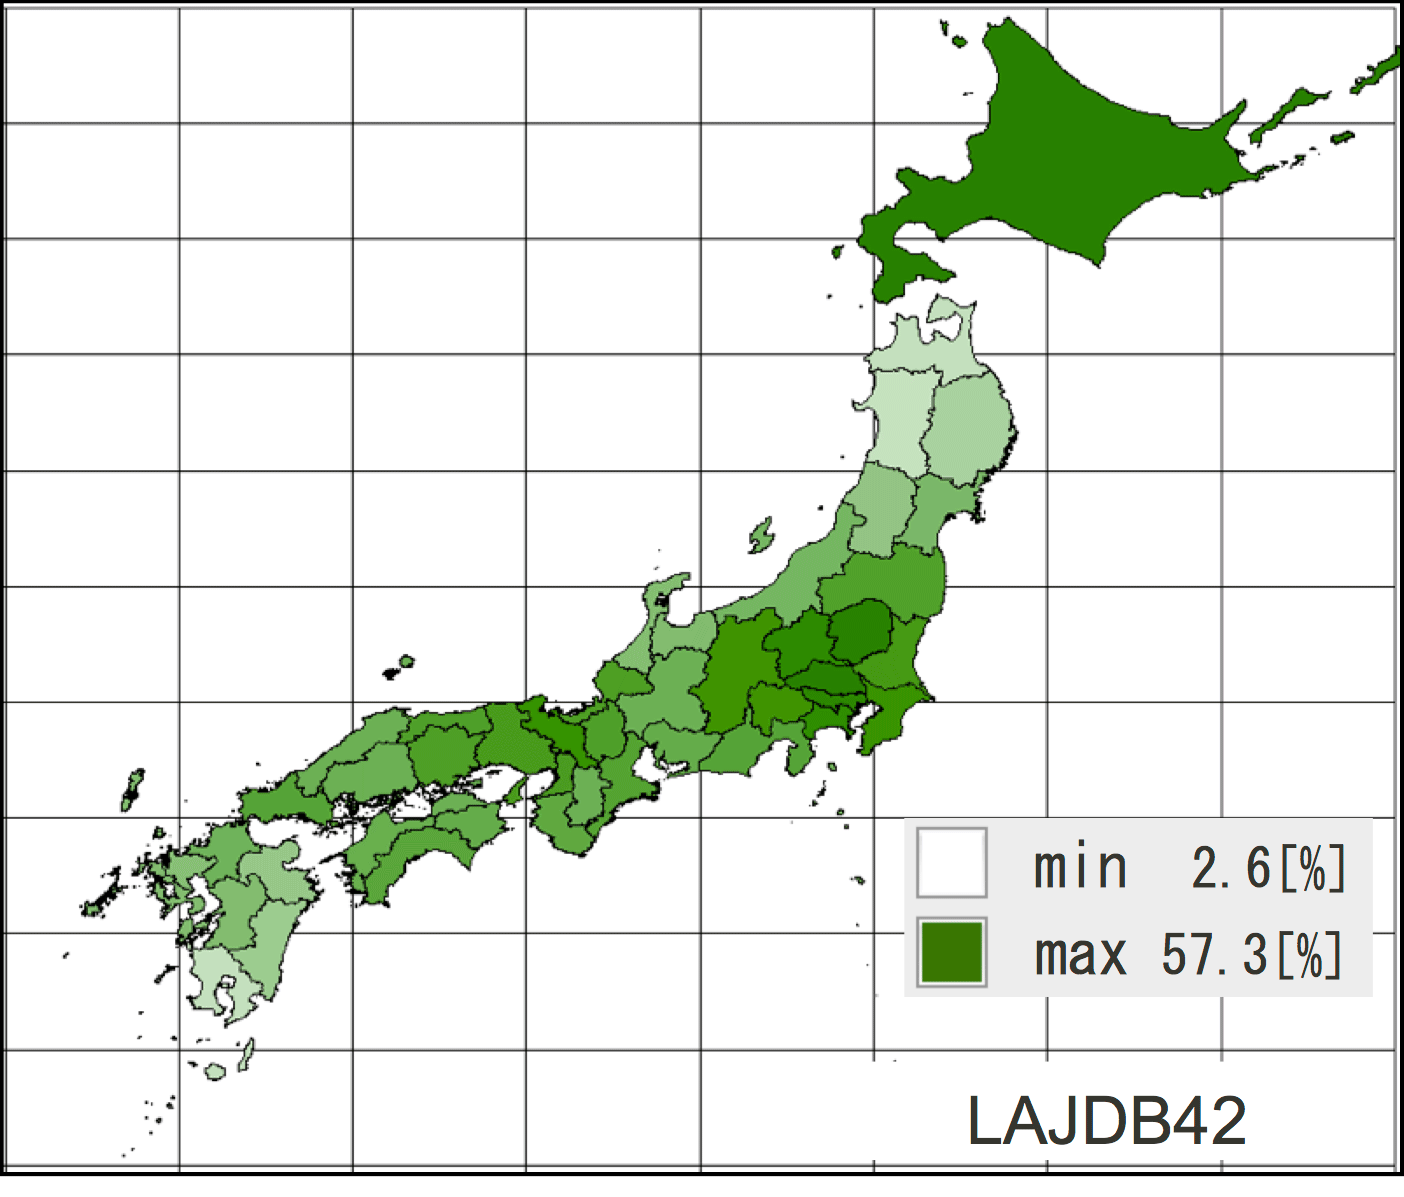
\includegraphics[width=0.8\textwidth]{illustrations/kuma_fig04}
\caption{Usage rates of standard forms of LAJDB42 data, summed up by prefecture.}          
\label{fig:4}
\end{figure} 

\begin{figure}
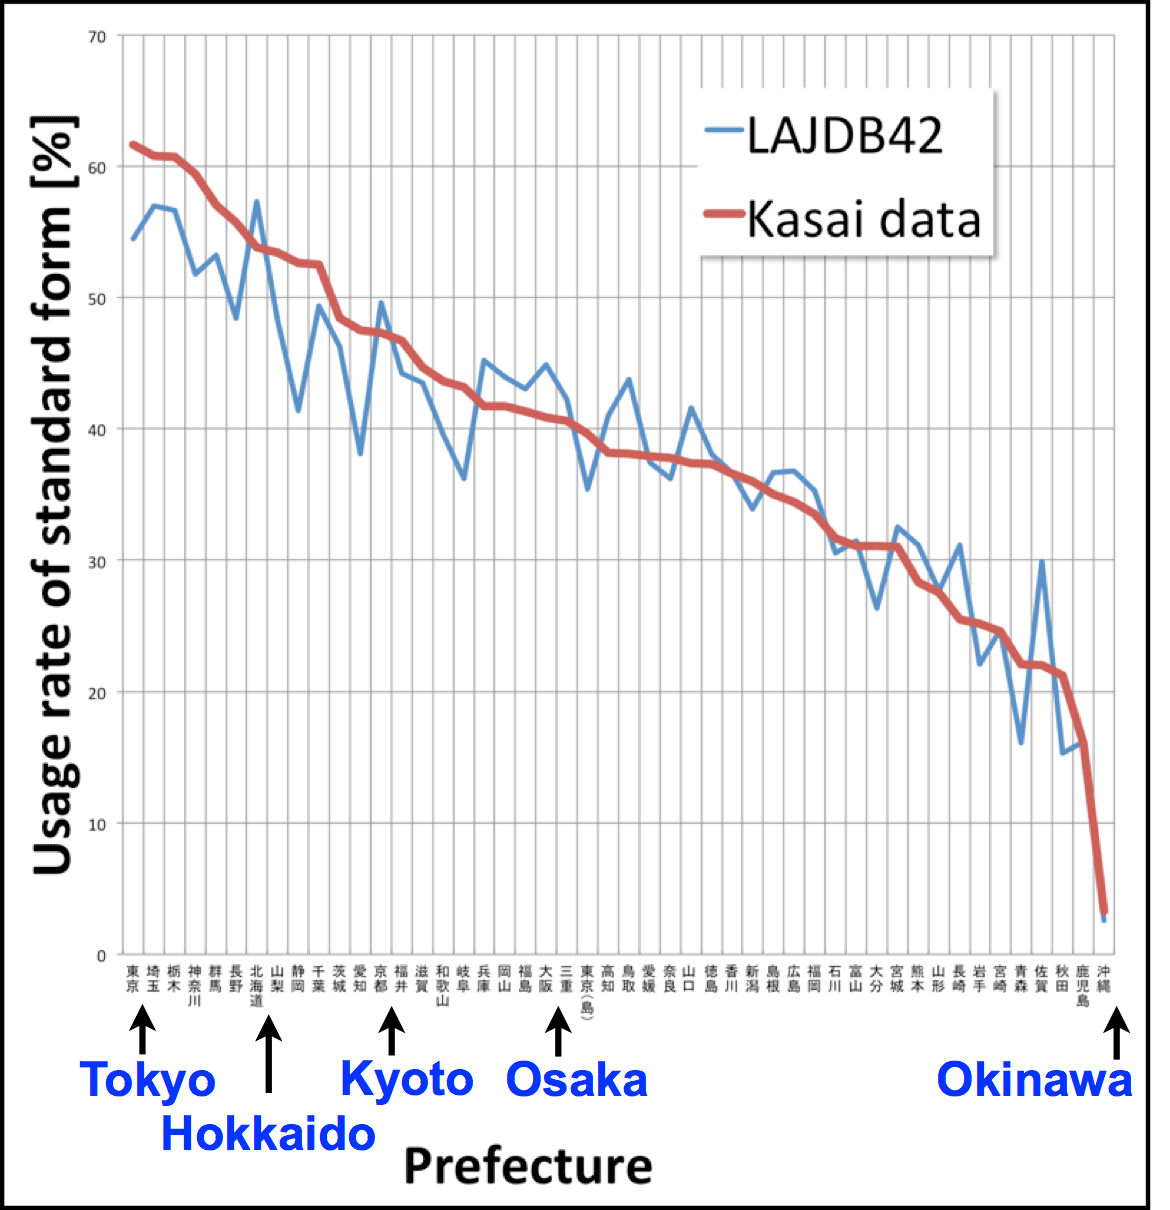
\includegraphics[width=0.8\textwidth]{illustrations/kuma_fig05}
\caption{Comparison between Kasai data and LAJDB42 data.}    
\label{fig:5}
\end{figure} 
\begin{figure}
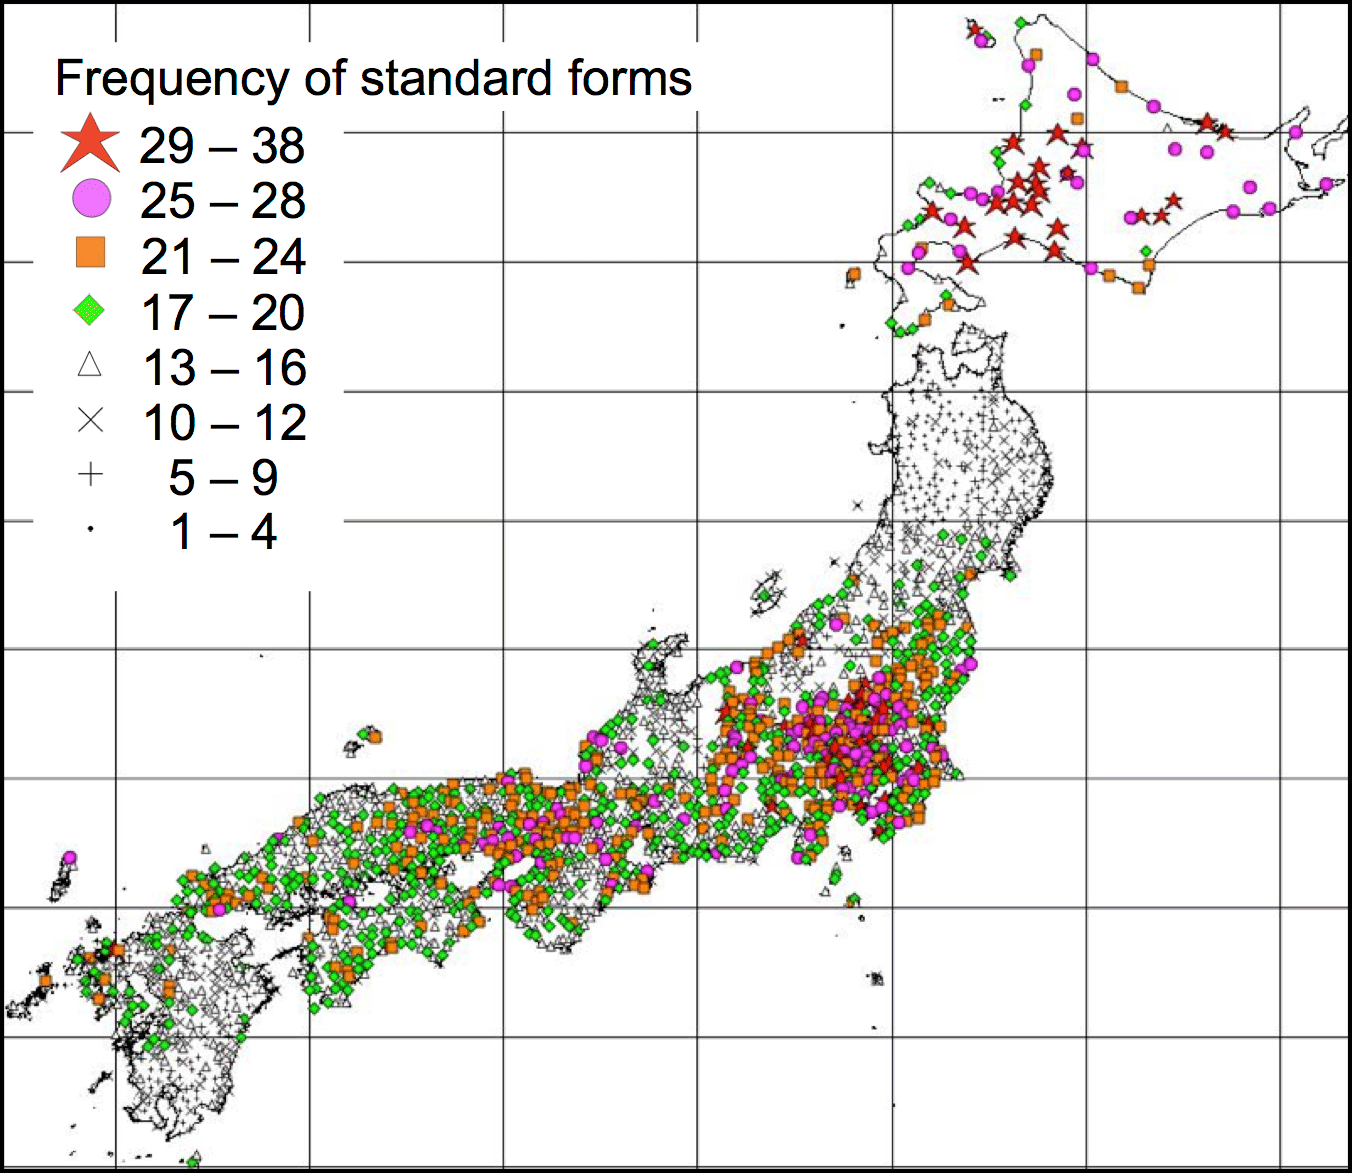
\includegraphics[width=0.8\textwidth]{illustrations/kuma_fig06}
\caption{Geographical distributions of frequency (GDF) of standard forms from LAJDB42 data.}          
\label{fig:6}
\end{figure} 

\figref{fig:7} shows the main roads in Japan in approximately 1885 (Honshu, Shikoku, and Kyushu areas). This map was created based on “Introductory Map V,”\footnote{ Here, it must be noted that “Introductory Map V: The main roads in Meiji period (around 1885)” aimed to provide an overview of the relationships between the surveyed localities and road networks. Roads were drawn on the basic map of the LAJ with reference to 1:200000 scale maps compiled via the Army Land Survey conducted by the General Staff of the Imperial Japanese Army (153 maps compiled and published from 1884 to 1893). The editors of the LAJ selected the national roads and prefectural roads that form the maps. The explanatory note stated that although there may be some roads that had been planned but not realized, “Introductory Map V” contained the most important roads around 1885. \figref{fig:7}, a digital map, was made by tracing the roads on “Introductory Map V,” and the projection system of the map from the LAJ was not explained in its documentation. Thus, the map shown in \figref{fig:7} is an approximation and involves some deviation (This map will be checked against the original compiled maps). Nonetheless, it is valuable and useful for explorative observation. Further, in the following observation, I consulted some related maps, books, and so on to confirm the observations. See also footnote~9.} a road map of the modern period, in the LAJ. An explanatory note from the LAJ states that this map provides an overview of land transport at the time during which the informants were growing up. This historical map is useful for comparing land transport—an important extra-linguistic factor—with dialect distributions. (Certainly, other means of transportation existed, but they were excluded as items for future incorporation into studies of the LAJ.) The thick purple lines denote the national roads, and the thin blue lines denote the prefectural roads.

\begin{figure}
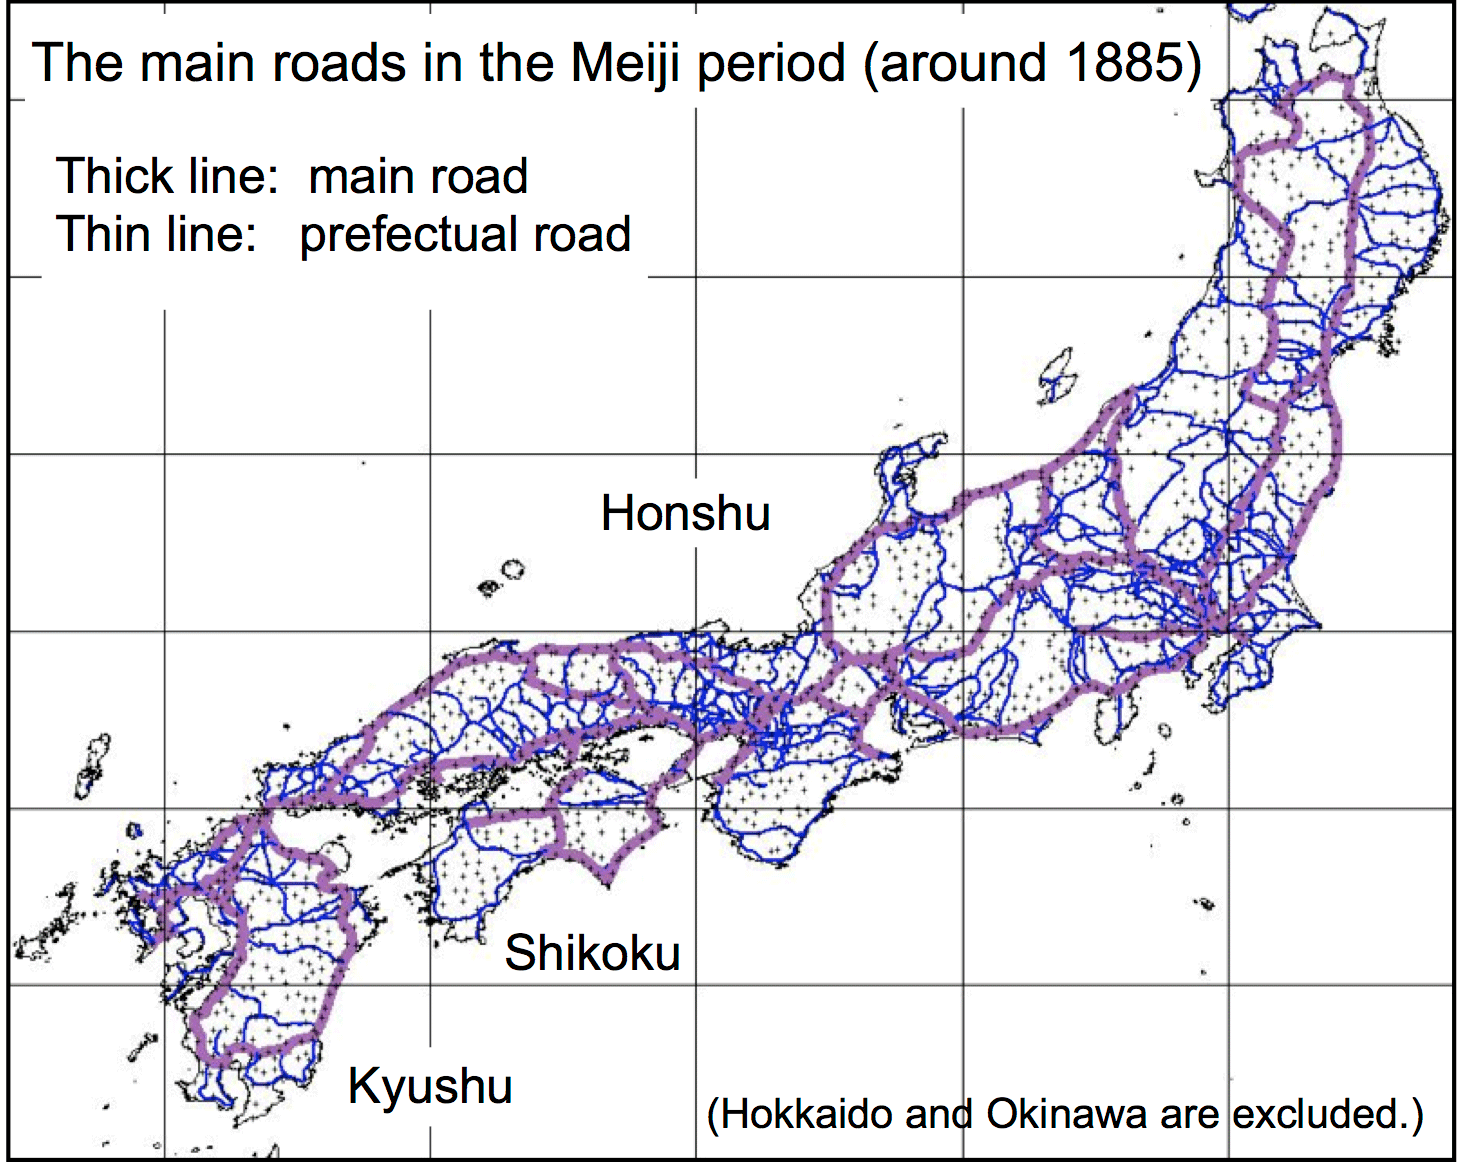
\includegraphics[width=0.8\textwidth]{illustrations/kuma_fig07}
\caption{The main roads in the Meiji period (around 1885, Honshu, Shikoku, Kyushu areas).}          
\label{fig:7}
\end{figure} 
\begin{figure}
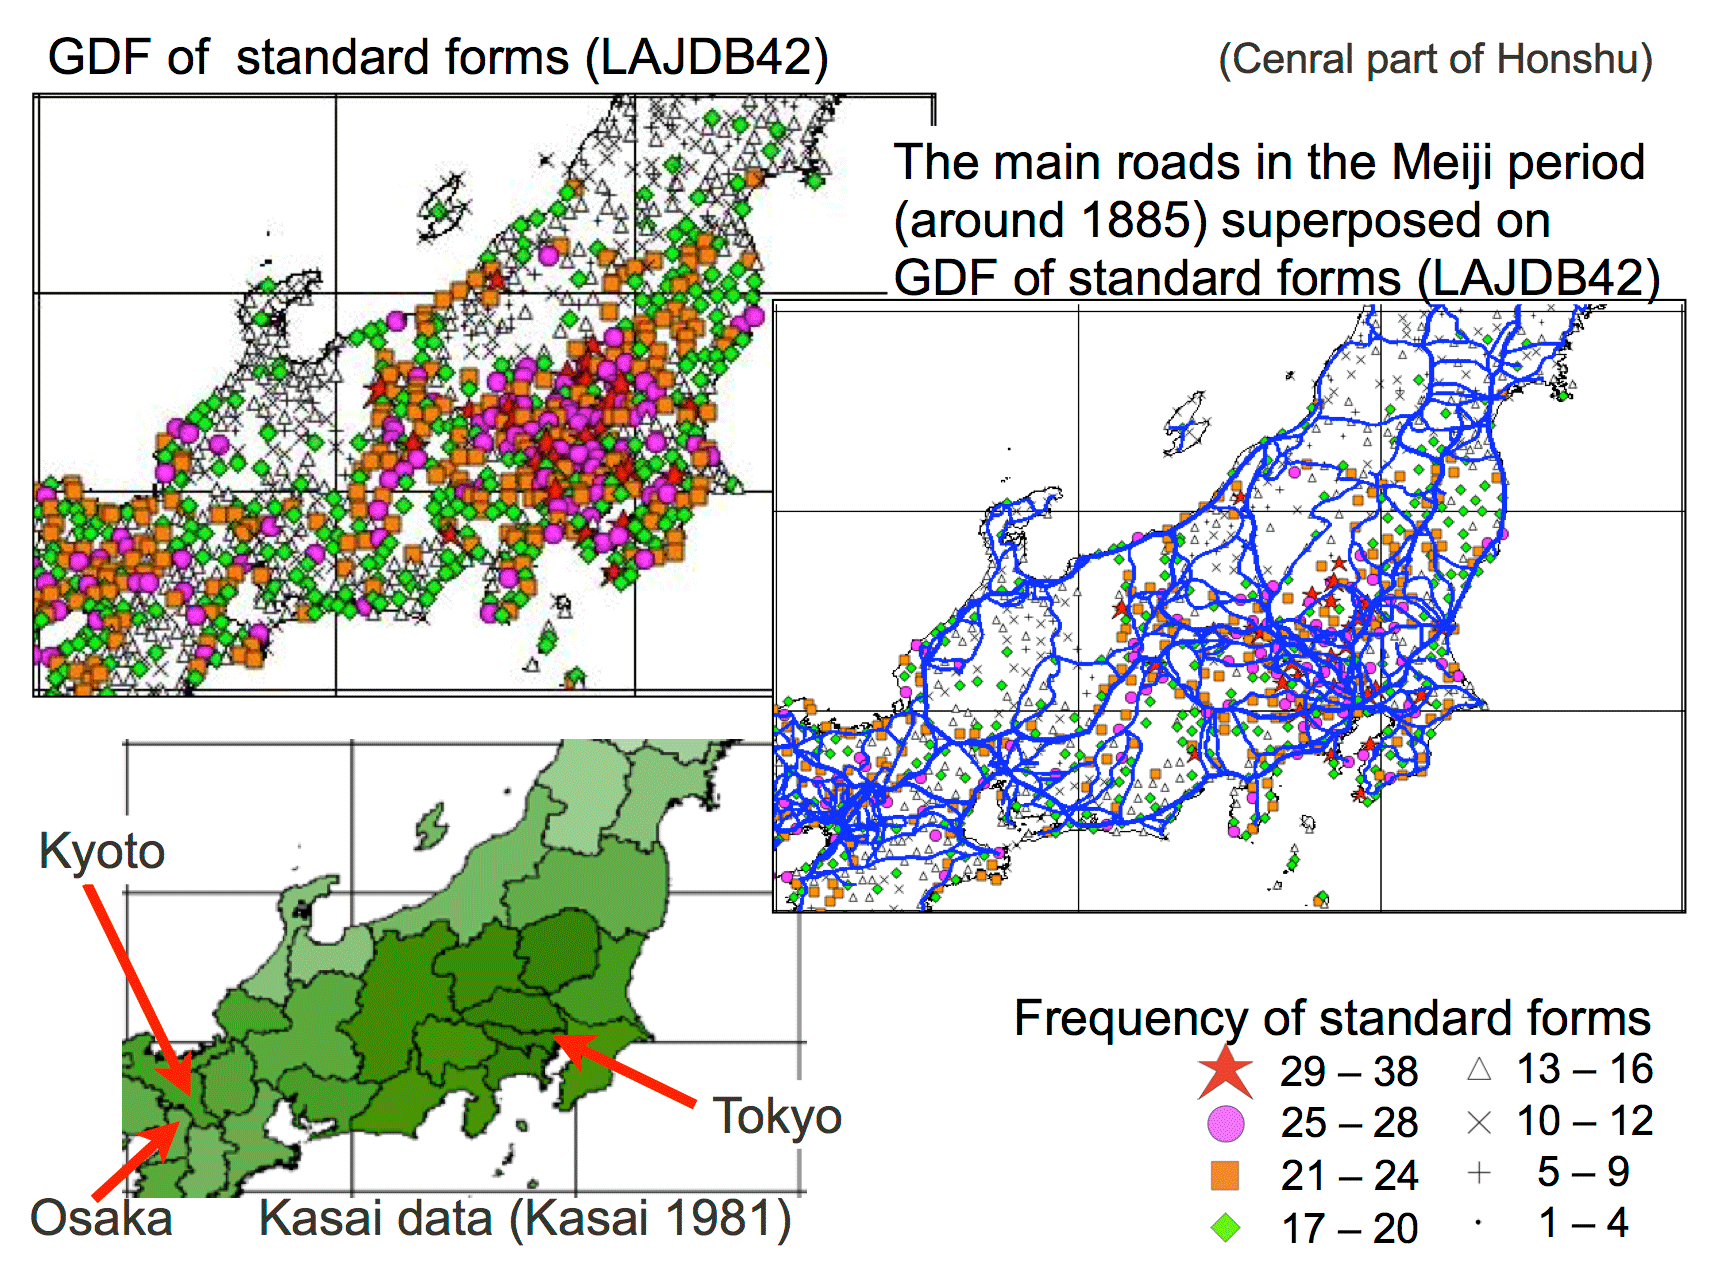
\includegraphics[width=0.8\textwidth]{illustrations/kuma_fig08}
\caption{Comparison between \figref{fig:6} and \figref{fig:7} (Central part of Honshu).}          
\label{fig:8}
\end{figure} 

Now let us see the relation between the main roads and geographical distributions of the frequency of standard forms. To illustrate this relation more precisely, \figref{fig:8} focuses on the central part of the Honshu area, which includes Tokyo (the current capital city) and Kyoto (the former capital city). The roads are superimposed on the distributions of the frequency of standard forms. Interesting observations can be formed regarding the relation between the distributions and the roads.

The map in \figref{fig:9} includes Tokyo (current capital), Kyoto (former capital), and Osaka (large commercial city). The roads connecting Tokyo, Kyoto, and Osaka are very important. There are main roads (“Kaido”), side roads (“Waki-kaido”), and others. Tokaido and Nakasendo are the two major main roads connecting these principal cities (Figures 11 and 12). Based on the Kasai data mentioned previously (see \figref{fig:3}), \citet[184]{tanaka_hyojungo:_1991} observed that the distribution of relative high frequency usage rates along the Tokaido route is interesting and noteworthy. The Nakasendo route runs through the mountainous areas, and Tokaido was the route used by feudal lords in the Edo period (17th century to the middle of the 18th century) to travel to Edo (present Tokyo). The Japanese tend to consider the Tokaido route rather than the Nakasendo route as the major road connecting Tokyo and Kyoto. However, based on LAJDB42 data, the Nakasendo route stands out. Localities with a high frequency of standard forms are plotted along the Nakasendo route. Comparisons drawn between the Tokaido and Nakasendo routes produce interesting results. Future studies on transportation history facilitate deeper insights pertaining to this observation.

\begin{figure}
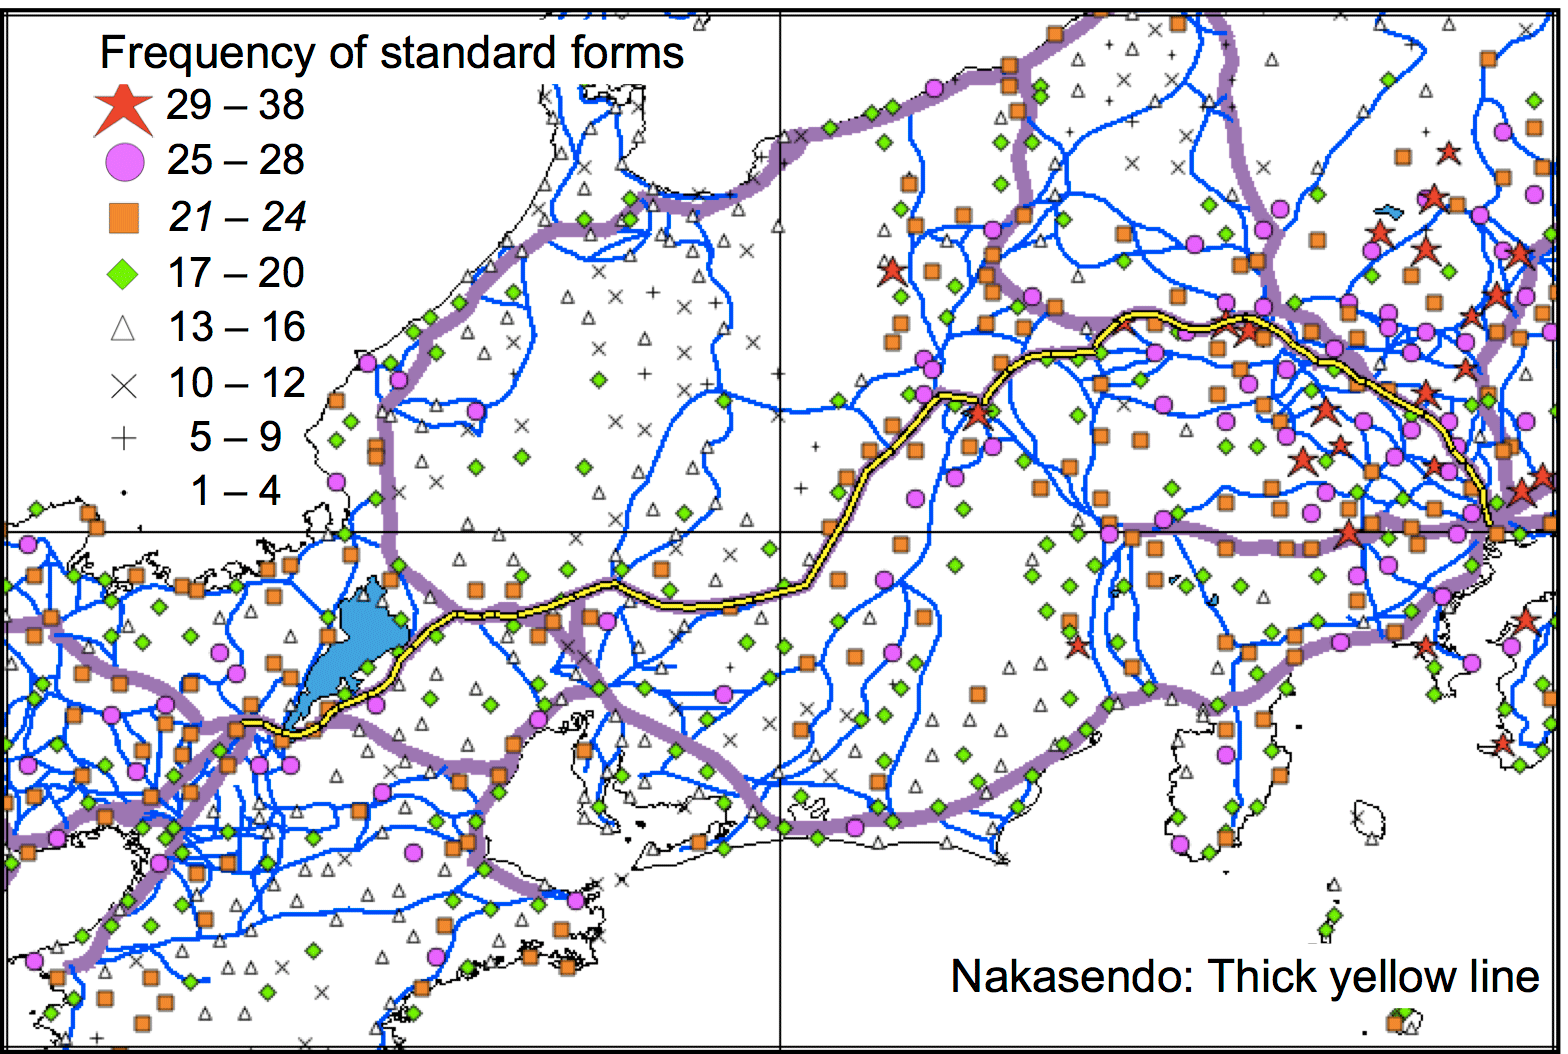
\includegraphics[width=0.8\textwidth]{illustrations/kuma_fig09}
\caption{GDF of standard forms superimposed on the main roads in the Meiji period [Nakasendo].}          
\label{fig:9}
\end{figure}

\begin{figure}
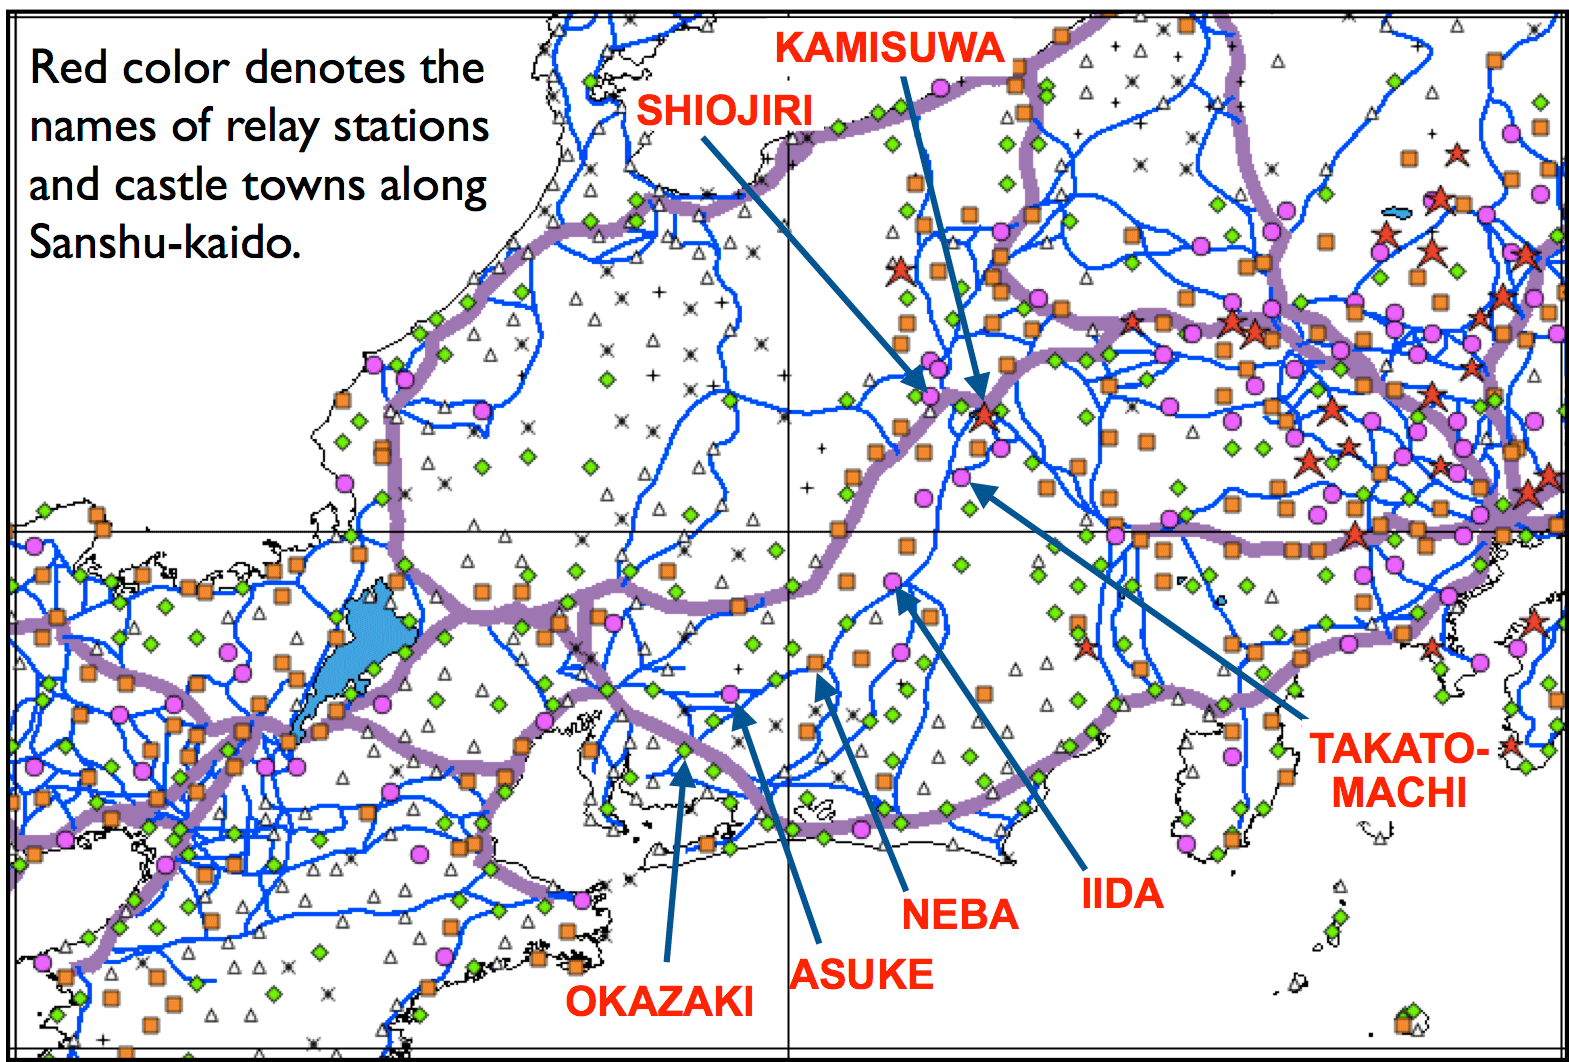
\includegraphics[width=0.8\textwidth]{illustrations/kuma_fig10}
\caption{GDF of standard forms superimposed on the main roads in the Meiji period [Sanshu--kaido].}          
\label{fig:10}
\end{figure}

\begin{figure}
\centering
\begin{subfigure}{.45\textwidth}
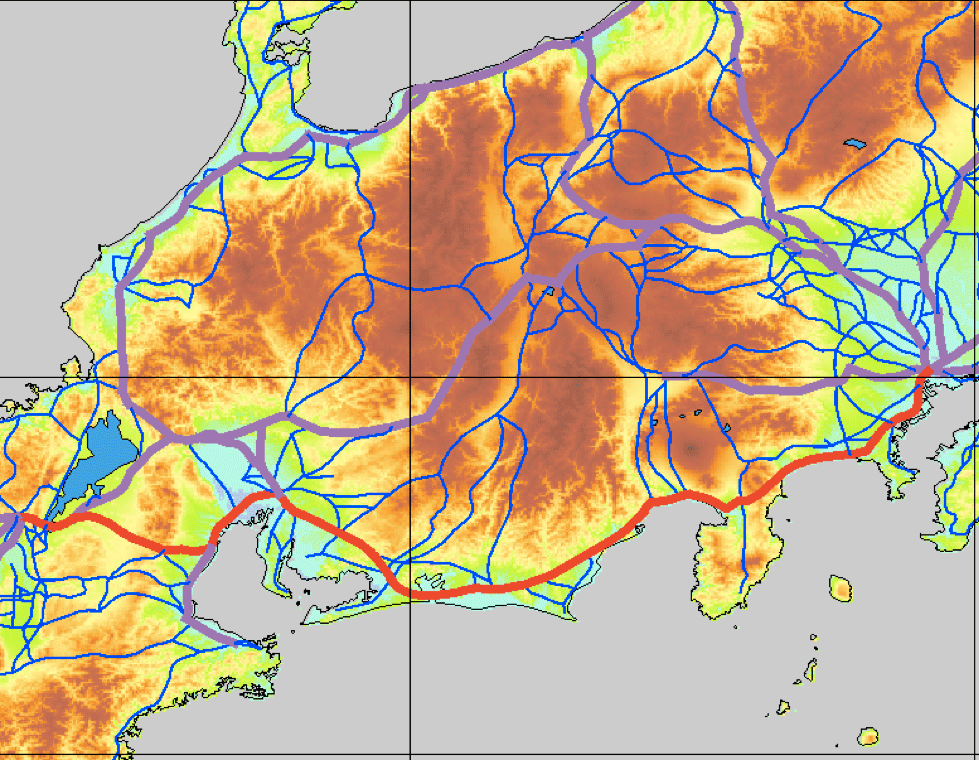
\includegraphics[width=1\textwidth]{illustrations/kuma_fig11}
%\caption{Tokaido route.}          
\label{fig:11}
\end{subfigure}~
\begin{subfigure}{.45\textwidth}
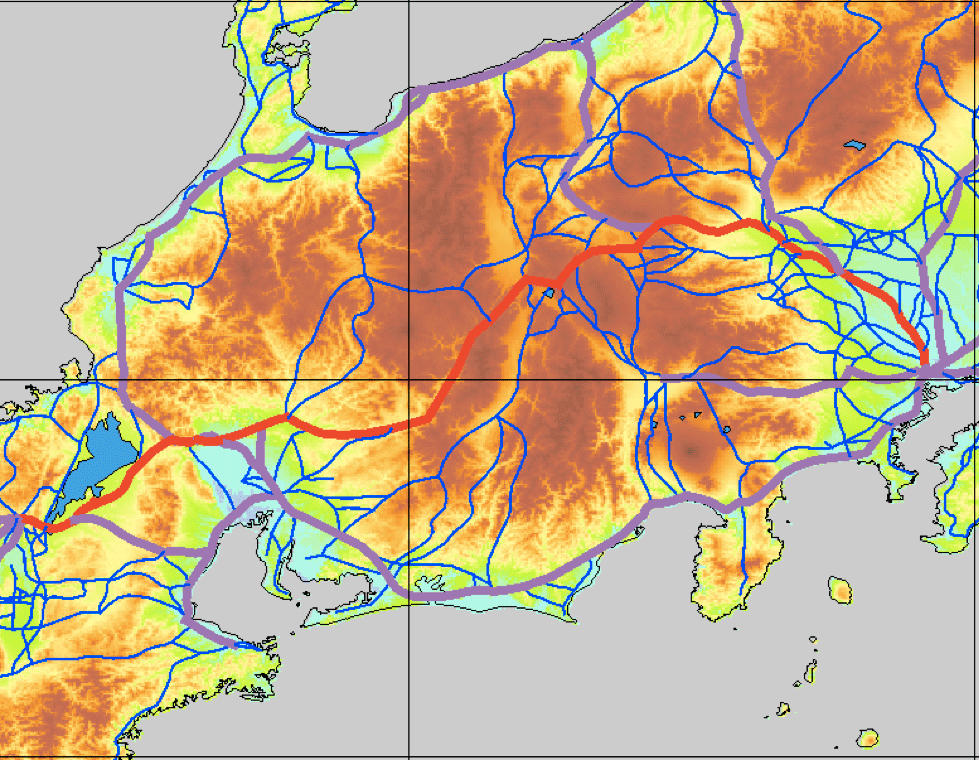
\includegraphics[width=1\textwidth]{illustrations/kuma_fig12}
%\caption{Nakasendo route.}          
\label{fig:12}
\end{subfigure}
\caption{Left: Tokaido route. Right: Nakasendo route.}
\end{figure}

\begin{figure}
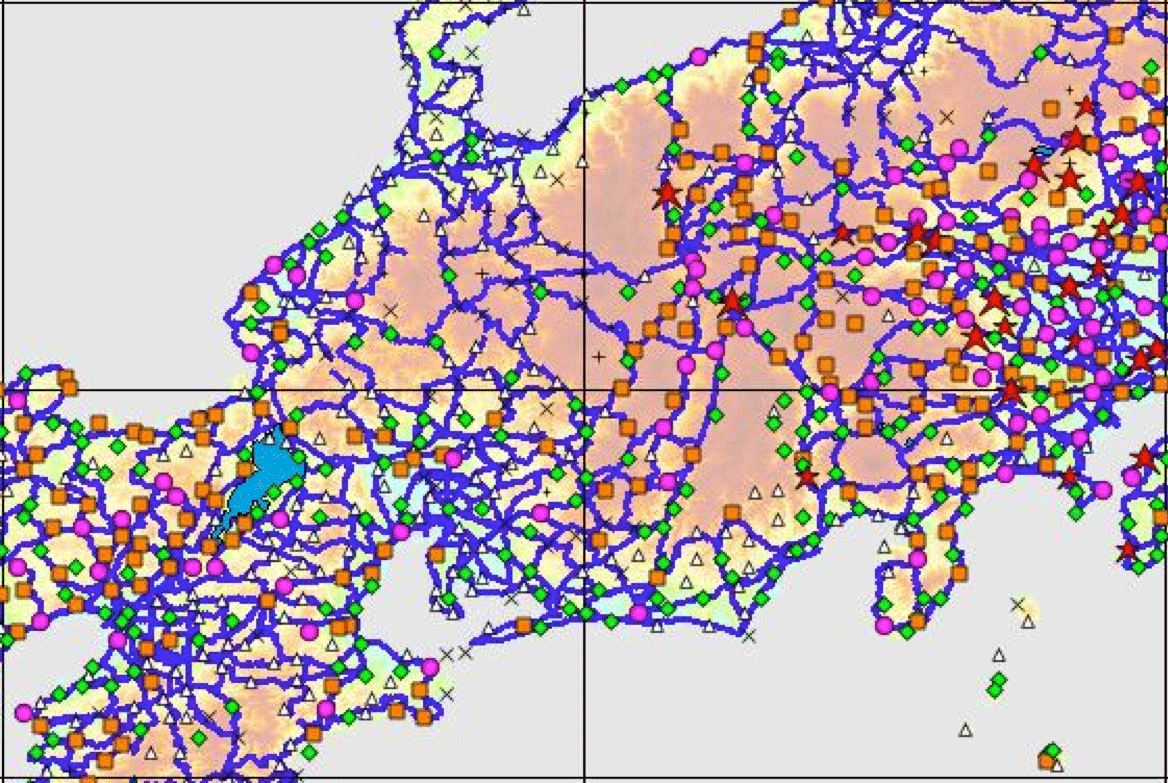
\includegraphics[width=0.8\textwidth]{illustrations/kuma_fig13}
\caption{GDF of standard forms superimposed on current road network.}          
\label{fig:13}
\end{figure}

Another interesting example is Sanshu-kaido, a side road of Nakasendo. Sanshu-kaido is a route that connects Shiojiri, Iida, Neba, Asuke, and Okazaki (\figref{fig:10}). Similar to the Nakasendo route, Sanshu-kaido appears prominent, with localities with a high frequency of standard forms observed along this route.\footnote{\figref{fig:13} shows the geographical distributions of frequency of standard forms superimposed on the primary route at present (around 2010). This map is prepared for double-checking. The localities with a high frequency of standard forms along Sanshu-kaido coincide with the route better in this map (see footnote 8). It must be noted that new roads are sometimes built along old roads and other times are not. As a whole, this observation also supports the observation above. Road network data: Geospatial Information Authority of Japan (2011); Global Map Japan in Global Map ver. 2.0. Elevation data: Geospatial Information Authority of Japan (2000); Global Map Japan in Global Map ver. 1.0.} Sanshu-kaido is not a major road; instead, it was developed as a road for transporting goods. Further systematic observations and analysis should lead to more interesting findings. Notably, these observations were not possible based on the former prefecture-unit calculations of the LAJ.

\subsection{Geographical frequency distributions for multiple answers}
In some localities, two or more linguistic forms were recorded. These multiple answers play an important role in the interpretation of maps, as they form relations between language contacts, diffusions, and changes. \citet{inagaki_hogen_1980} provided some observations about multiple answers on a few maps from the LAJ, and \citet{inoue_heiyo_2004} noted the importance of these multiple answers and examined their position in the process of diffusion of standard forms. 

\begin{figure}
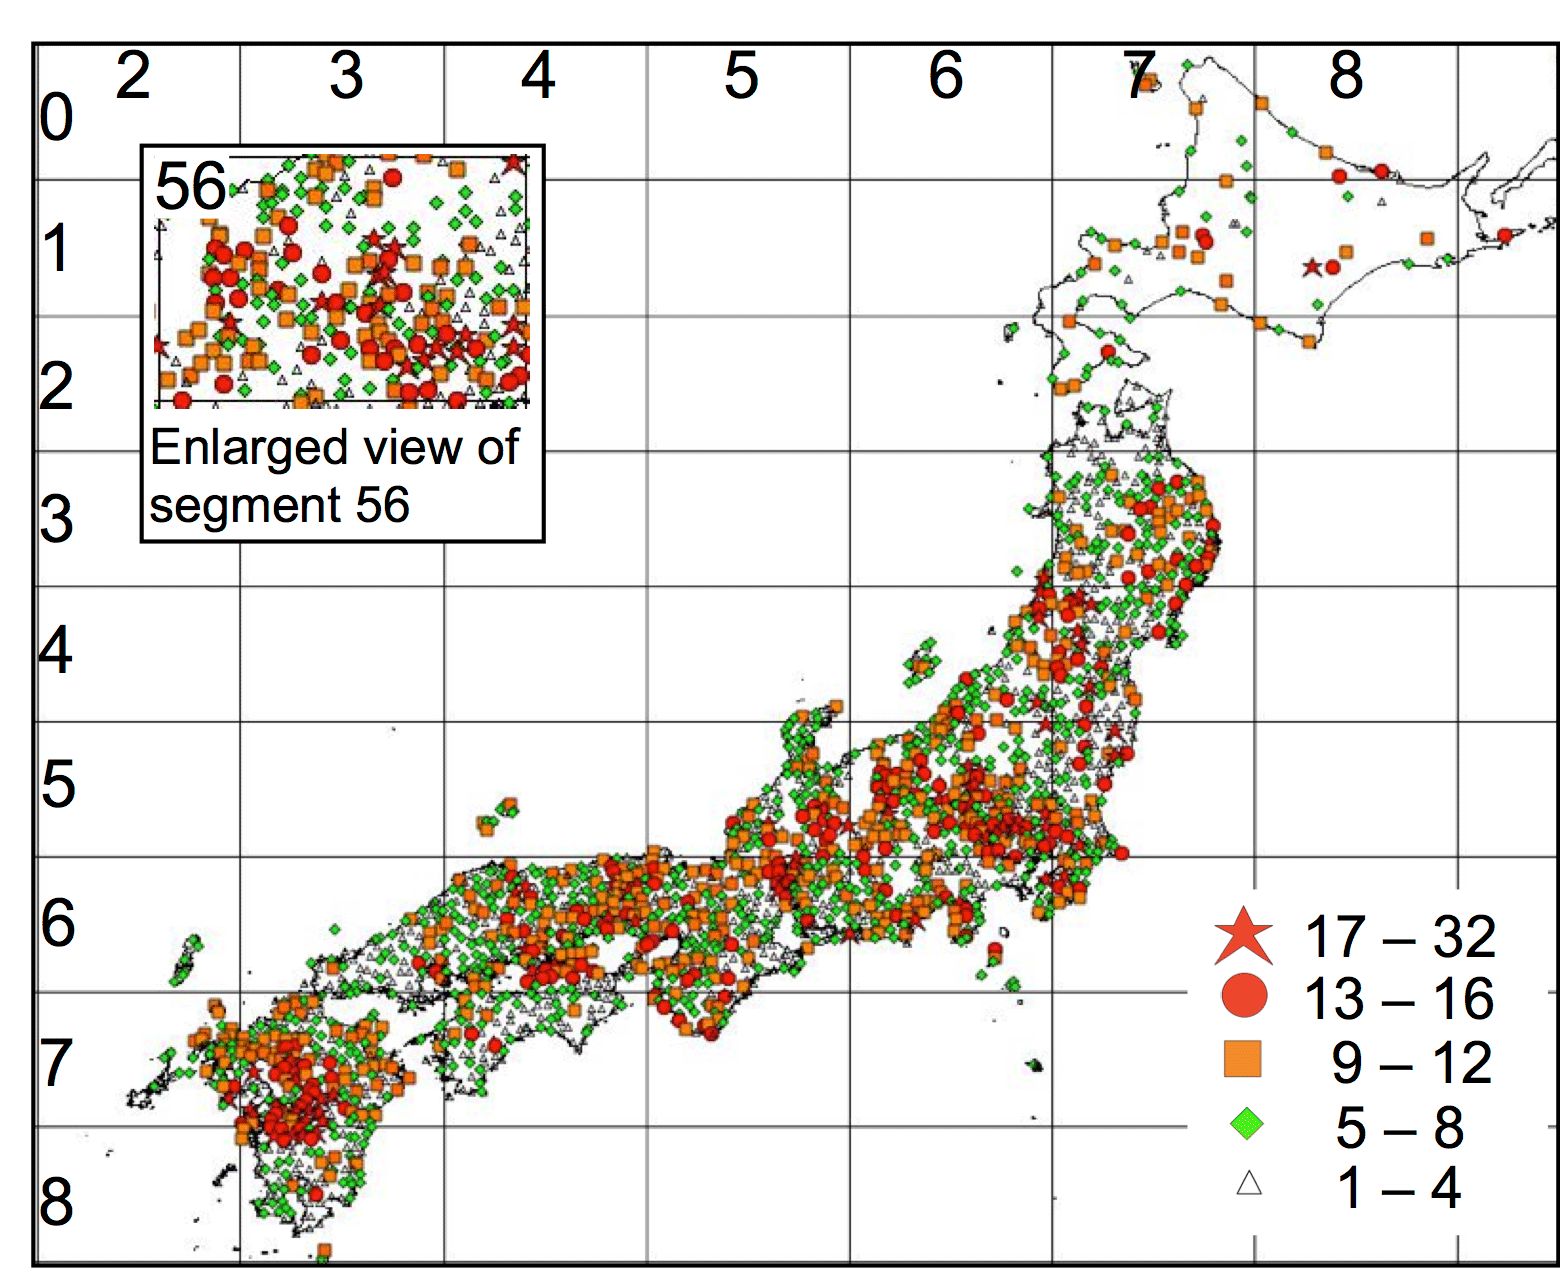
\includegraphics[width=0.8\textwidth]{illustrations/kuma_fig14}
\caption{GDF of multiple answers, LAJDB55.}          
\label{fig:14}
\end{figure}

\begin{figure}
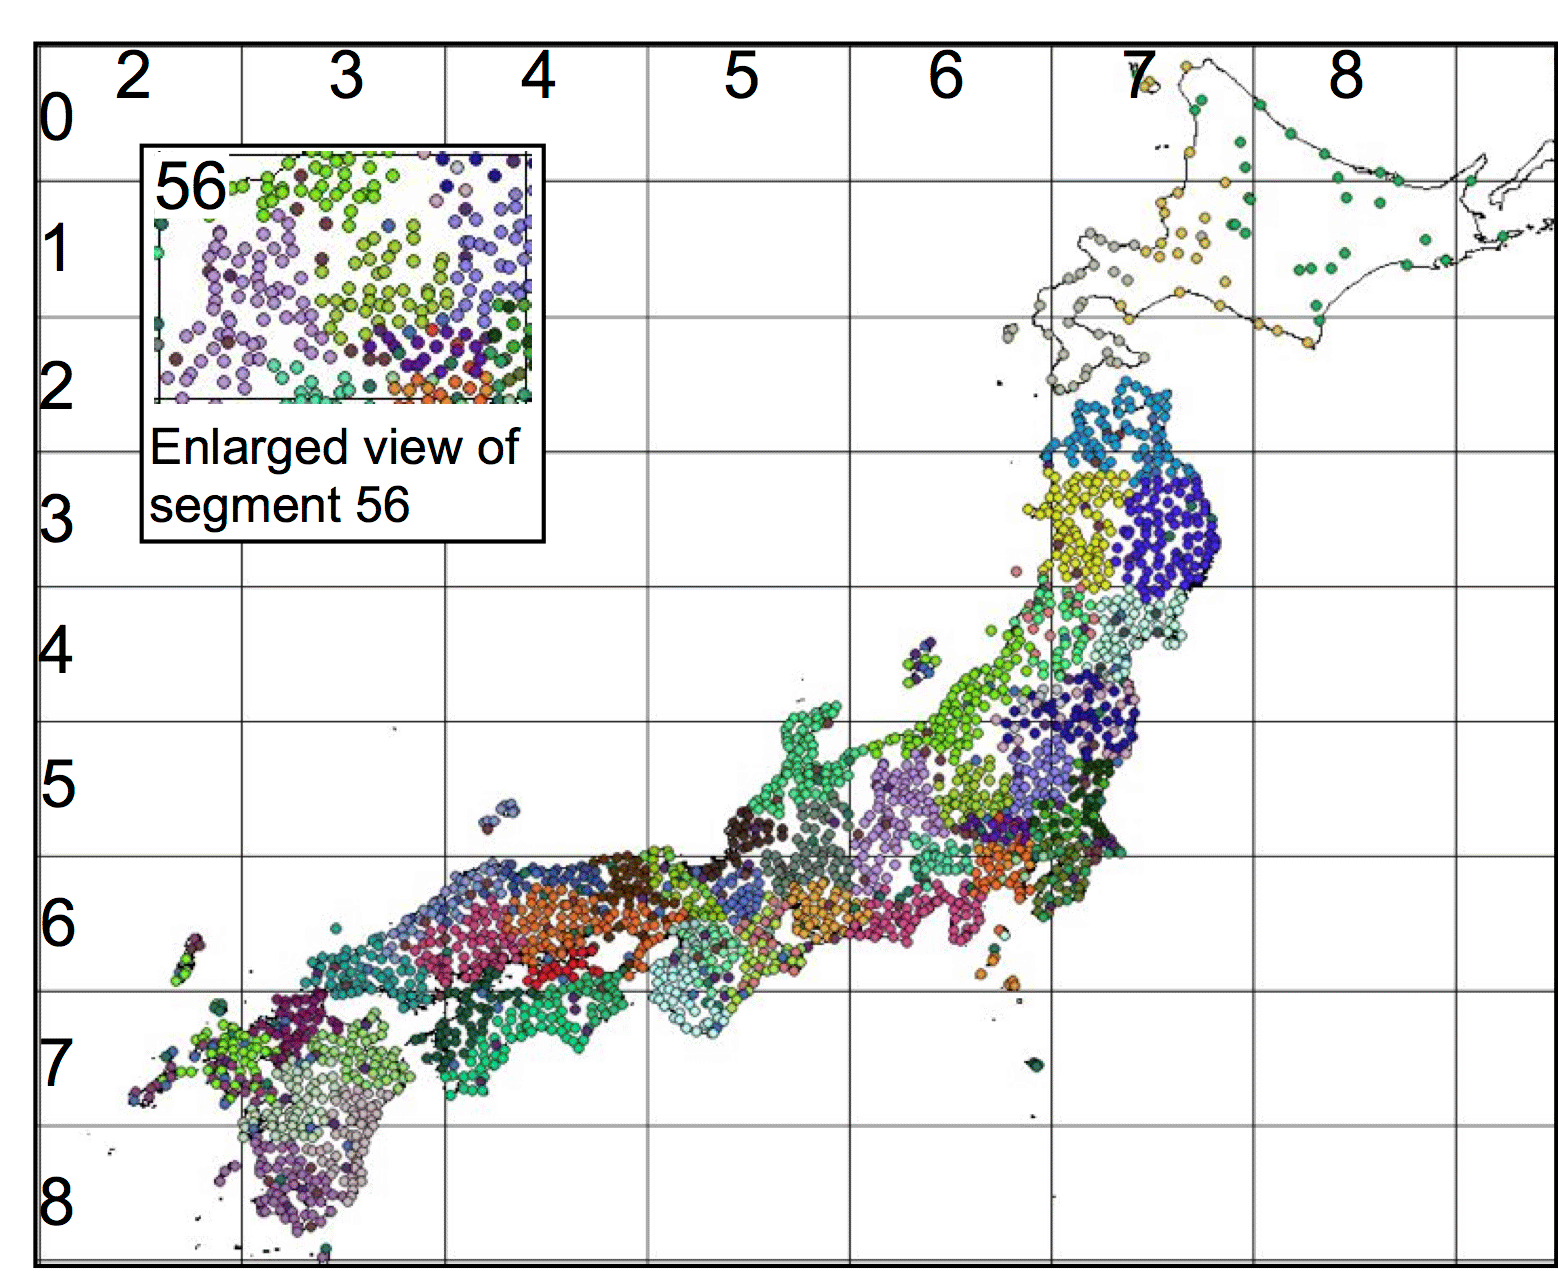
\includegraphics[width=0.8\textwidth]{illustrations/kuma_fig15}
\caption{Localities color-coded according to fieldworkers.}  \label{fig:15}
\end{figure}

Few quantitative studies examine the distribution of multiple answers, and the actual status in the LAJ was only partially examined. However, such studies can be easily conducted using computerized data. \figref{fig:14} shows the geographical distributions of the frequency of multiple answers. LAJDB55 data is used here. This distribution contains all items including standard forms. It shows a significant distribution and is not distributed randomly all over Japan. \figref{fig:15} shows the localities color-coded according to the fieldworkers. As Fumio Inoue noted,\footnote{ A comment by Fumio Inoue, recorded in \citet[6]{inagaki_hogen_1980}.} it is probable that some fieldworkers tended to record more multiple answers, while others tended to record fewer. As a rule, the LAJ survey was designed to maintain uniformity\footnote{ During the LAJ survey, to maintain uniformity in the fieldworker’s surveys, various attempts were incorporated into the survey design. For example, “to assure a greater uniformity in the questioning, one of the members of the directing dialect bureau from Tôkyô, accompanied the local fieldworkers during the survey of one or more of the assigned localities. The technique of selecting an informant and the method of questioning was then demonstrated.” Furthermore, “221 localities were surveyed by one of the directors” and “these localities are equally distributed over the whole territory,” \citep[23, 40--41]{kokuritsu_kokugo_kenkyujo_nlri_nihon_1966}.} among fieldworkers; however, it is important to be careful about such risks and verify the observations from multiple perspectives. Accordingly, I compared the distributions of the localities assigned to each fieldworker and the distributions of the frequency of multiple answers. We can see the continuous distribution patterns of the GDF of multiple answers, which spread beyond the boundaries of the fieldworkers’ distributions. In other words, we can observe that the boundaries do not limit the continuity of the distribution patterns of the GDF (see, e.g., the enlarged views in \figref{fig:14} and \figref{fig:15}).

\subsection{The frequency of informant’s comments on standard forms among multiple answers}
For the LAJ, the editors maintained a principle called the “principle of processing multiple answers.” When two linguistic forms were recorded in one locality, both were marked on the map. However, when one of the two forms was the standard language form and, in addition, this fact was noted by the informant—such as in the answers “This is a new polite form.” or “This is the word used in school.”—then the editors would omit the standard forms from a map. This method was followed because the LAJ survey aimed to record informants’ personal speech used in their familiar and daily surroundings. Certainly, dialectical forms identical with standard forms were not omitted if there were no informant comments. The principles for processing multiple answers to the LAJ are as follows.

\begin{quotation}
Further elements of interpretation are given by the informant’s comment (“old word,” “new form,” etc.) or by the fieldworker’s notes. These have been helpful for the map interpretation, and they will be published in a later volume.\footnote{The publication of comments and notes was not realized. Also see footnote 5.} When two linguistic forms have been recorded in the same locality, they have been both marked on the map. When, however, one of the two is the standard language form, and when, in addition, this fact has been noted by the informant (“this is the new polite form,” “this is the word used in the school,” etc.), in this case only, we have omitted the forms marked this way from the maps \citep[44]{kokuritsu_kokugo_kenkyujo_nlri_nihon_1966}.
\end{quotation}

To study the multiple answers, the omitted standard forms that informants had commented on (e.g., “This is new,” and so on) are important. In the course of compiling the LAJ, the editors assumed that the standard forms that were commented on as “new” were distributed randomly. However, using one LAJ item as an example, \citet[152--153]{sato_chiikishakai_1986} plotted the omitted answers on a map and found that by adding the omitted answers, the distribution pattern of the standard forms became clearer. However, this observation was based on only one item. The real state of the multiple answers of the LAJ is yet to be explored. Fumio Inoue\footnote{A comment by Fumio Inoue, recorded in \citet[5]{inagaki_hogen_1980}.} stated that the editors of the LAJ were aware of some regional differences of the standard forms that were commented on as new and considered these differences as interesting. However, the editors did not plot these words and were unsure about their significance. Using the LAJDB, it is possible to analyze the distribution of the word forms omitted from the atlas.

\begin{figure}
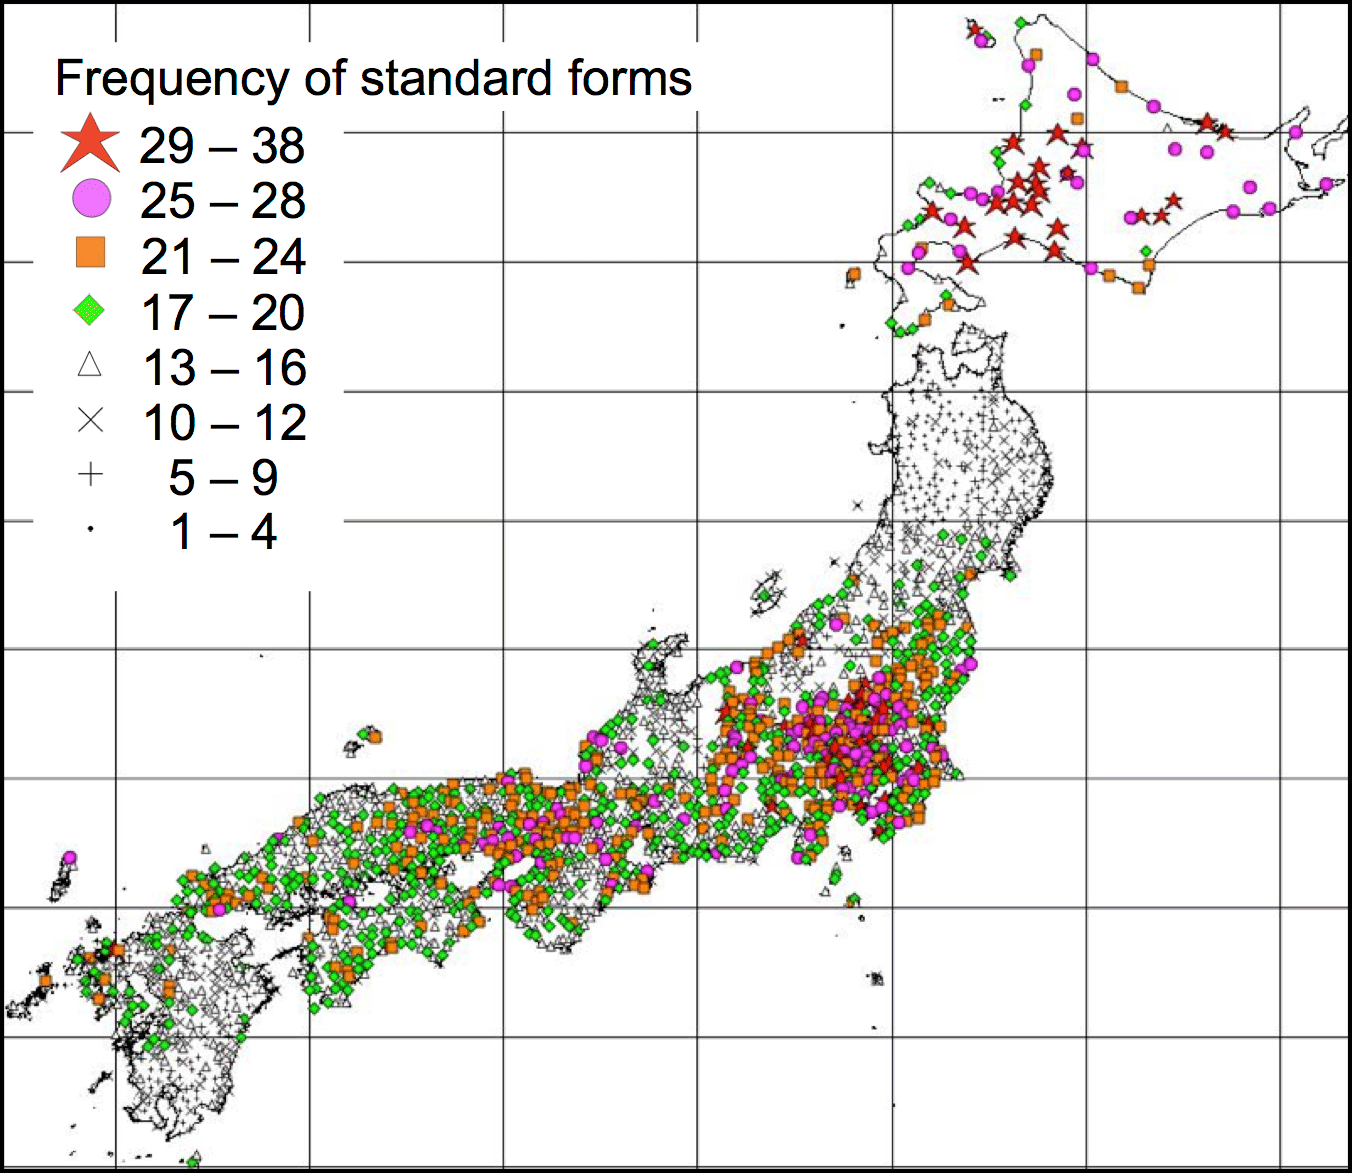
\includegraphics[width=0.49\textwidth]{illustrations/kuma_fig16-a}
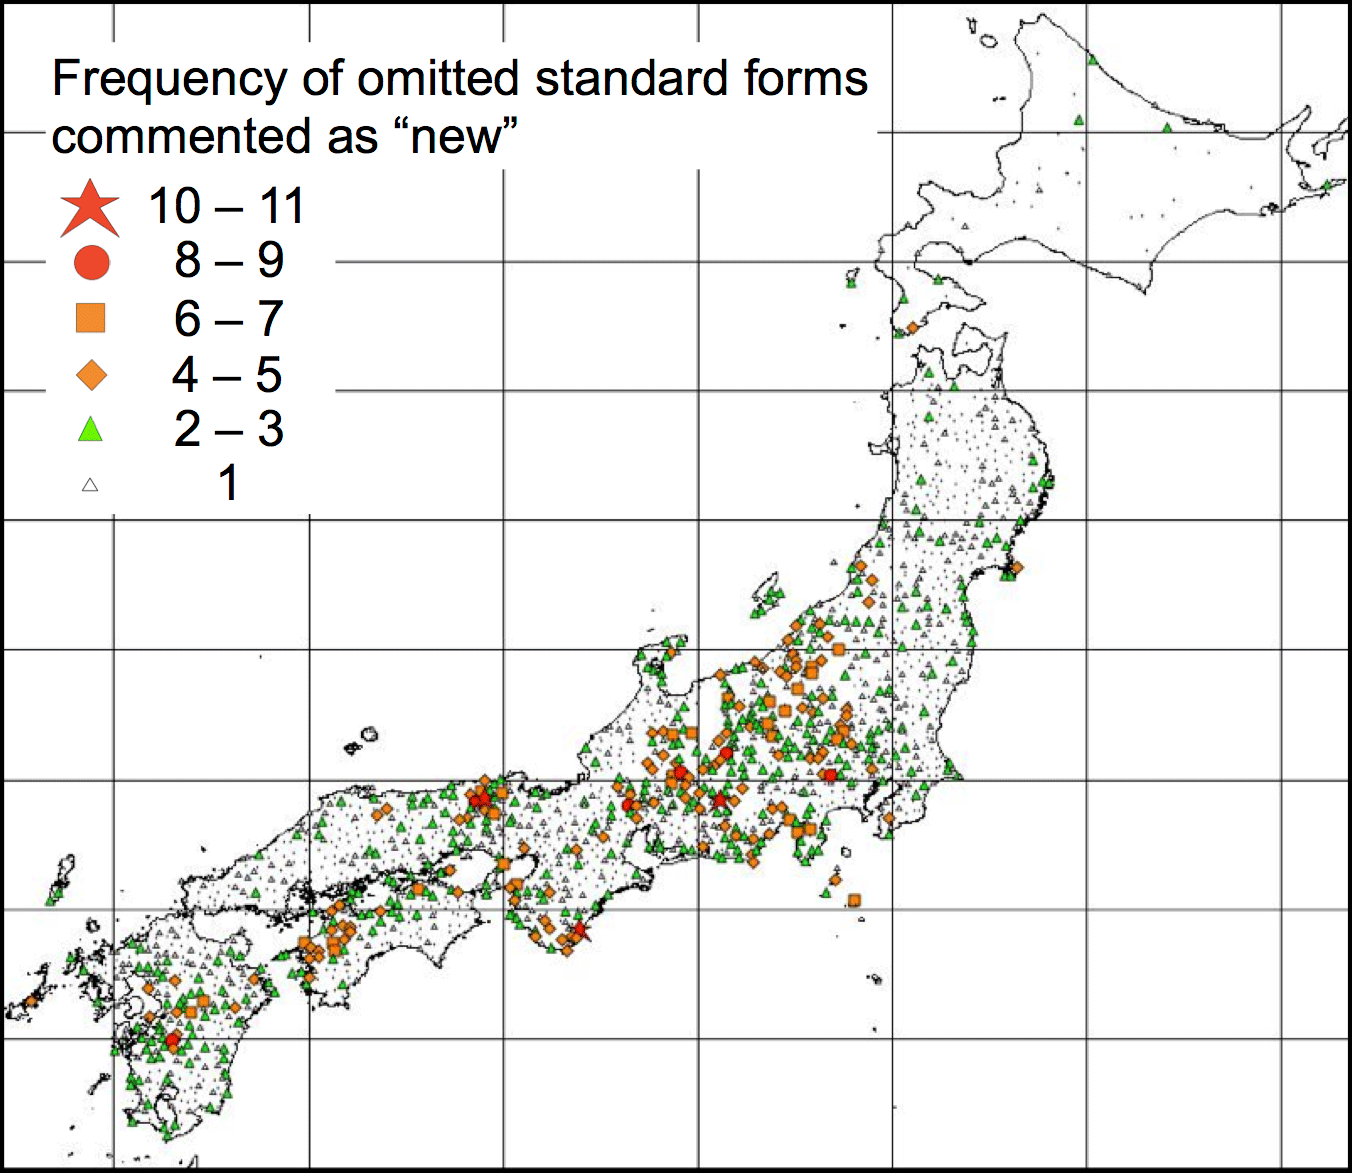
\includegraphics[width=0.49\textwidth]{illustrations/kuma_fig16-b}
\caption{Comparison between GDF of standard forms and omitted standard forms. Left: GDF of standard forms. Right: GDF of omitted standard forms commented as “new”.}          
\label{fig:16}
\end{figure}
% (a) GDF of standard forms (b) GDF of omitted standard forms commented as “new”\\

\begin{figure}
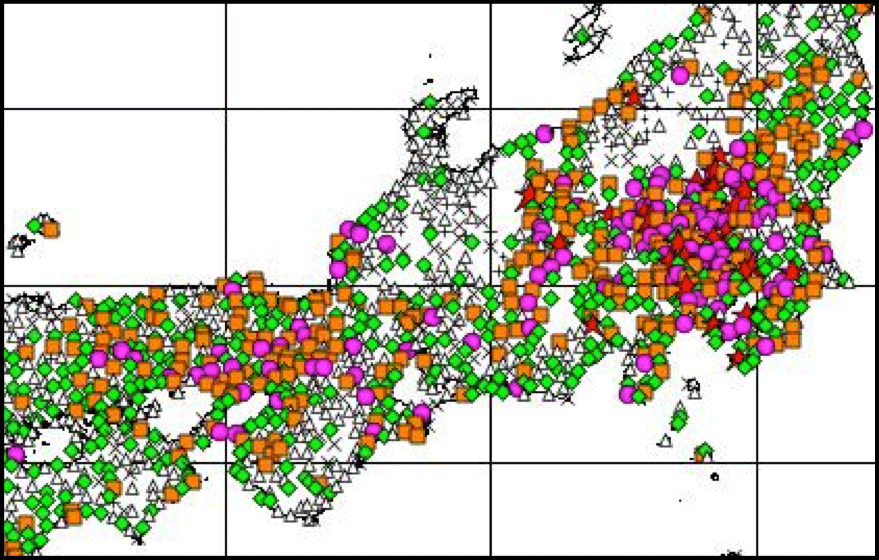
\includegraphics[width=0.49\textwidth]{illustrations/kuma_fig17-a}
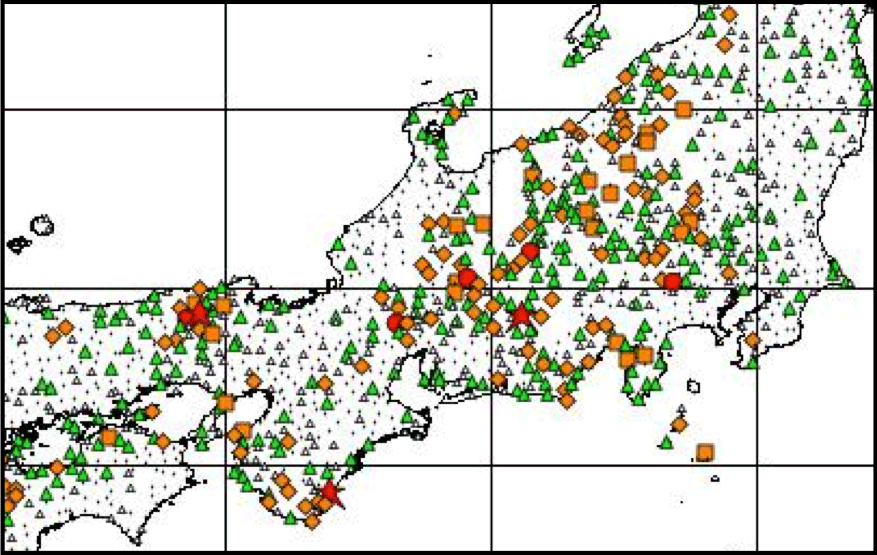
\includegraphics[width=0.49\textwidth]{illustrations/kuma_fig17-b}
\caption{Comparison between GDF of standard forms and omitted standard forms (Central Honshu). Left: GDF of standard forms. Right: GDF of omitted standard forms commented as “new”.}          
\label{fig:17}
\end{figure}
% (a) GDF of standard forms (b) GDF of omitted standard forms commented as “new”\\
 
On the card images provided by the LAJDB, we can see the omitted words and the editors’ markings, which signify the application of the principle of processing the multiple answers. In addition, there are lists of localities which record the notes, extracted from the original material cards, with some information about the word omissions performed by the editors. Based on these notes, I formulated data on the omitted word forms using LAJDB42. \figref{fig:16} shows the geographical distribution of the frequency of standard forms and that of omitted standard forms for comparison. Is there any relation between the distribution of the standard forms and the distribution of omitted standard forms? To observe this relation more precisely, \figref{fig:17} provides a zoomed-in image. By displaying these two maps alternately as an animation, we compared these two maps visually. For our observation, we focused on the Kinki area and the area surrounding it (\figref{fig:18}). 

\begin{figure}
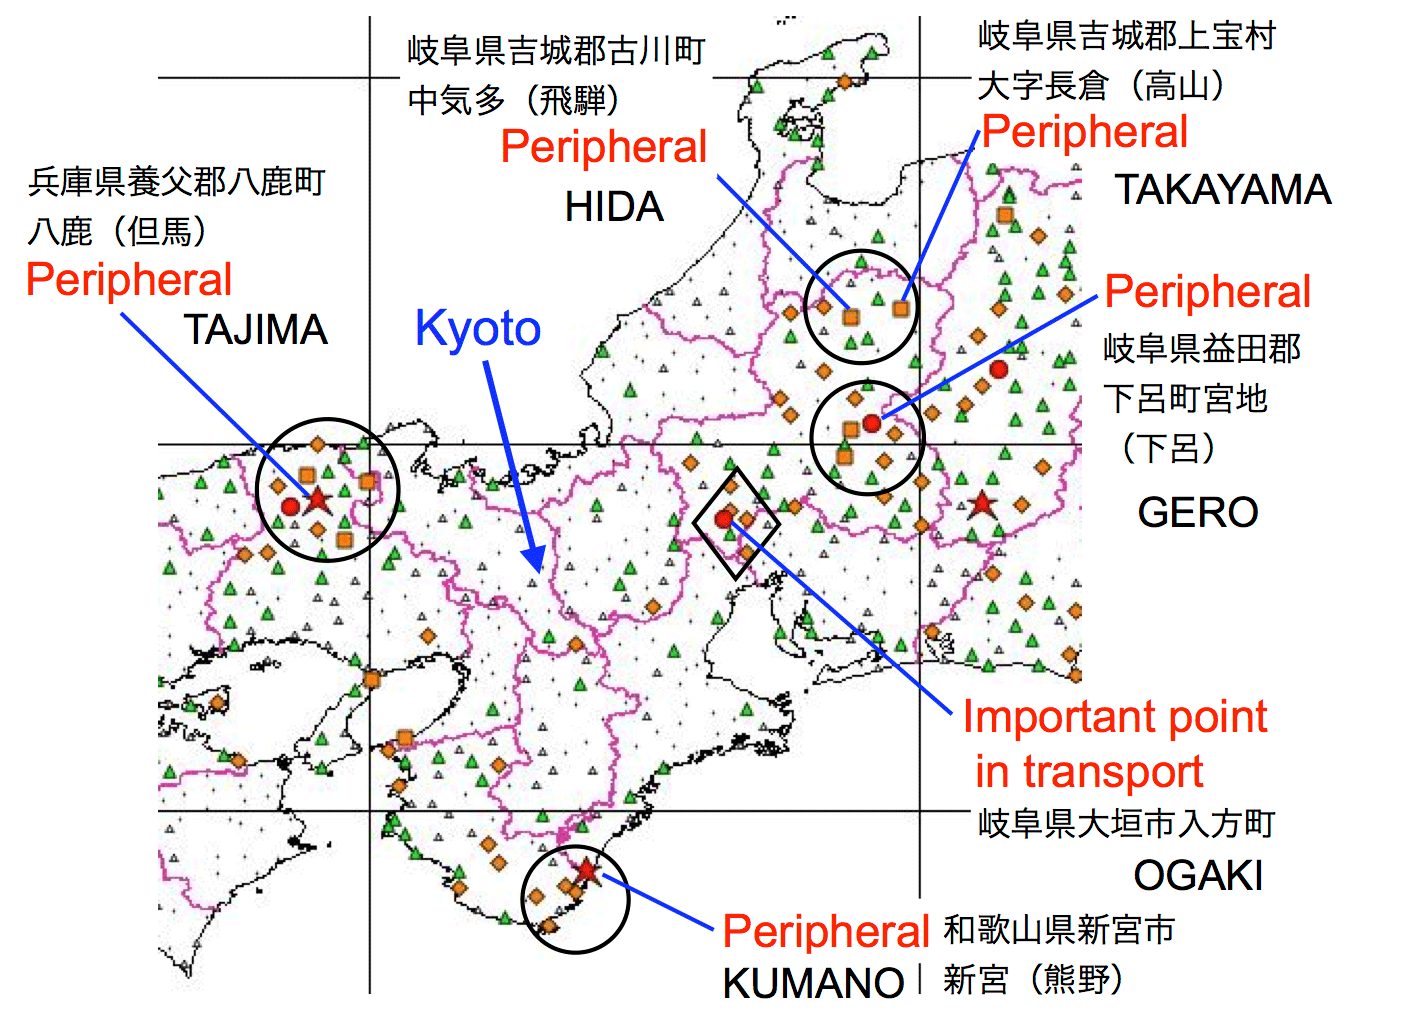
\includegraphics[width=0.8\textwidth]{illustrations/kuma_fig18}
\caption{GDF of omitted standard forms commented as “new” (Kinki area).}          
\label{fig:18}
\end{figure}

\begin{figure}
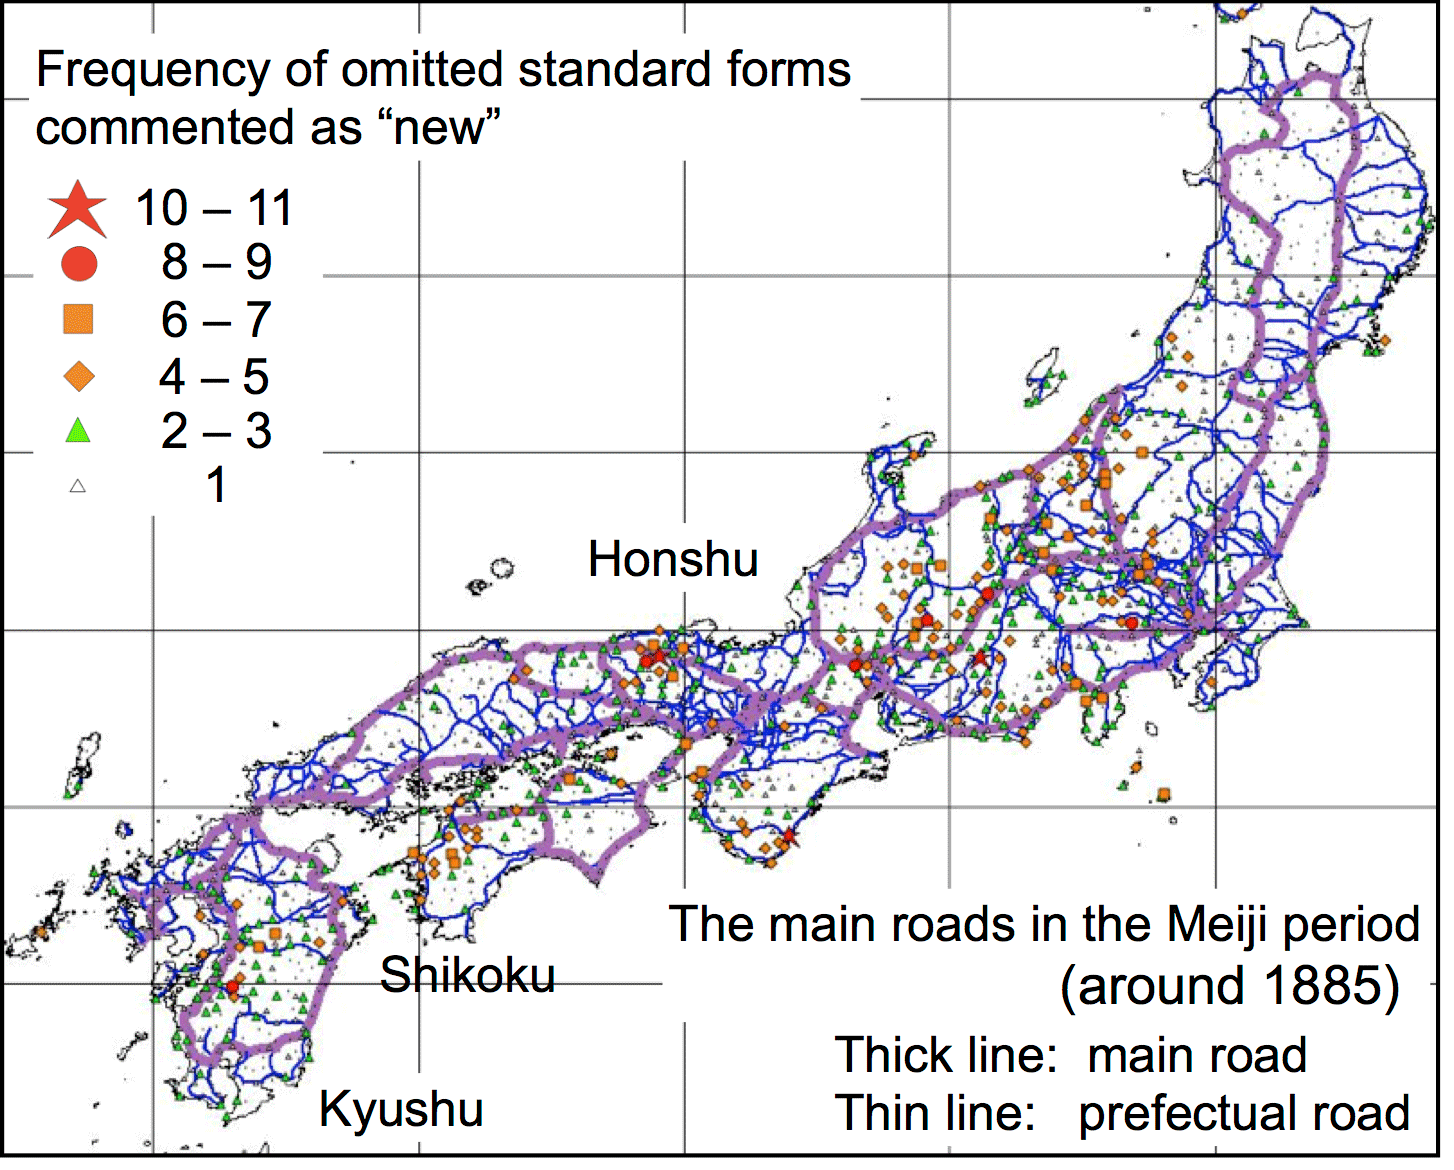
\includegraphics[width=0.8\textwidth]{illustrations/kuma_fig19}
\caption{GDF of omitted standard forms superimposed on the main roads in the Meiji period.}          
\label{fig:19}
\end{figure}             

\figref{fig:18} shows that in areas marked by circles, the areas where standard forms are frequently omitted are surrounded by or adjacent to those where standard forms are very frequent. In areas marked by a diamond shape, the high frequency areas of the two distributions are overlapped. Localities indicated by arrows show the highest frequency in each area marked above. The places marked by circles are the typical peripheral areas. The places marked by diamonds are important areas for transport. In this case, the marked places are clearly separated into two types. Although further investigation is required for other places, these indications are interesting. Possibly, the circled places are at the forefront of the diffusion of the standard forms. More studies should be conducted on areas indicated by diamond shapes.

\figref{fig:19} shows the geographical distribution of the frequency of omitted standard forms superimposed on the main roads in the Meiji period (approximately 1885). Further systematic observations and analysis should present interesting findings. Studies on the history of transportation and other types of knowledge of the regions will be helpful for further studies.

\subsection{ Geographical distributions of degrees of similarity}
In this section, the linguistic similarities among the localities based on the LAJDB data will be provided. This information will help present an overall image of the linguistic similarities spread over Japan based on the LAJ. LAJDB55 is used in this section. The previous observations were made mainly with reference to the standard forms. The following maps are based on all word forms including the standard forms. Here, linguistic similarity between two localities is measured by the number of linguistic features shared by the localities. The measure of linguistic similarity used is referred to as NC, that is, a number of common linguistic features. In this paper, NC denotes a number of common word forms (the NC between any two localities is calculated by adding the total number of the same word forms of each item in a dataset). \figref{fig:20} provides some examples\footnote{At the Methods XV conference, the geographical distributions of similarities were represented using animation (total number of frames or maps was 2400). In this case, similarity maps are played after they are sorted by locality number. This animation shows the maps in quick succession. This is an impressionistic form of representation; nevertheless, it allows for observation of reoccurring patterns, transition of patterns, and so on. Such a method of observation should be utilized as an exploratory tool. \figref{fig:20} provides some samples of similarity maps.} of geographical distributions of the degrees of similarities. A higher NC value corresponds to a larger radius of circle points. The red points are reference points.

\begin{figure}
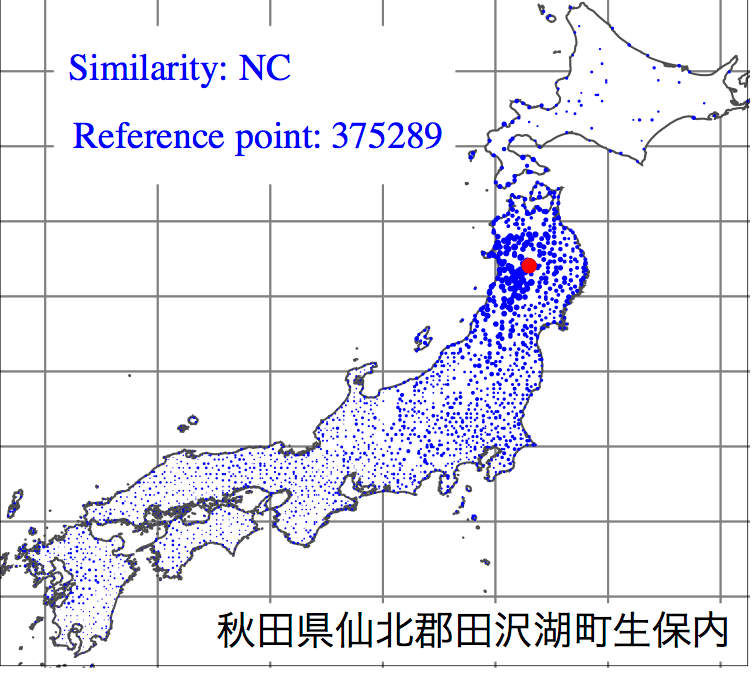
\includegraphics[width=0.32\textwidth]{illustrations/kuma_fig20-1}
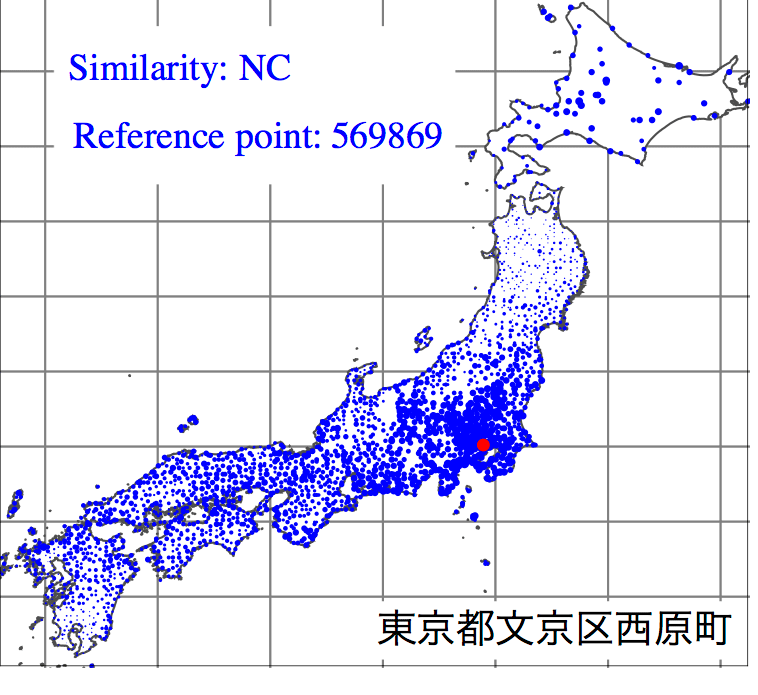
\includegraphics[width=0.32\textwidth]{illustrations/kuma_fig20-2}
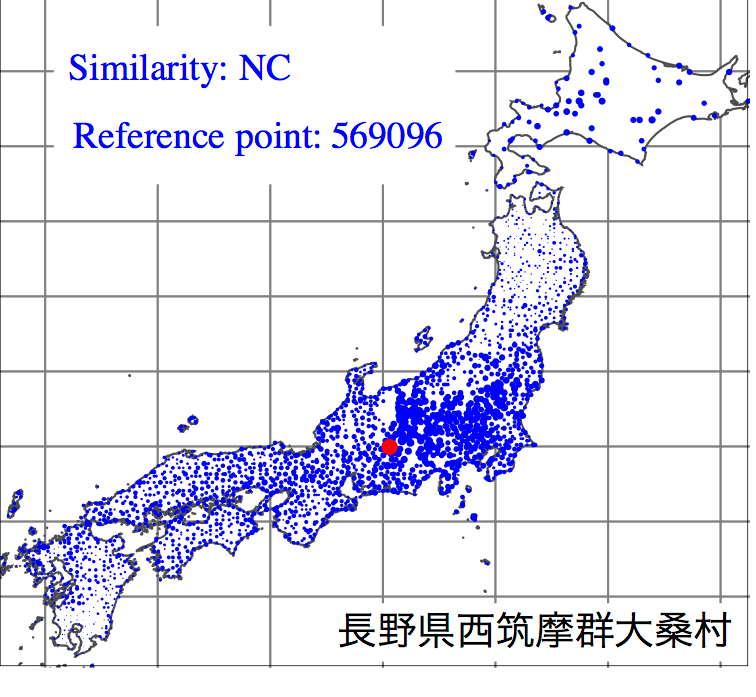
\includegraphics[width=0.32\textwidth]{illustrations/kuma_fig20-3}
\\
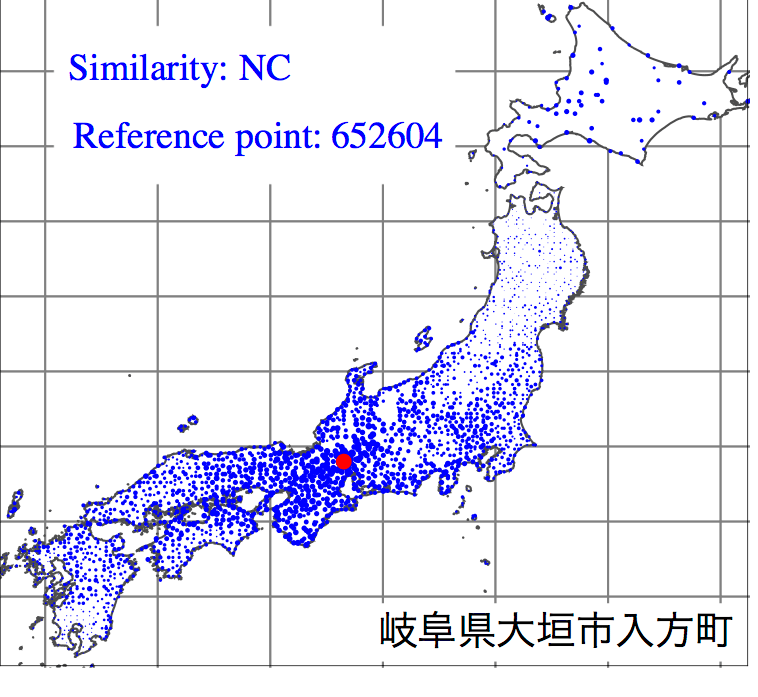
\includegraphics[width=0.32\textwidth]{illustrations/kuma_fig20-4}
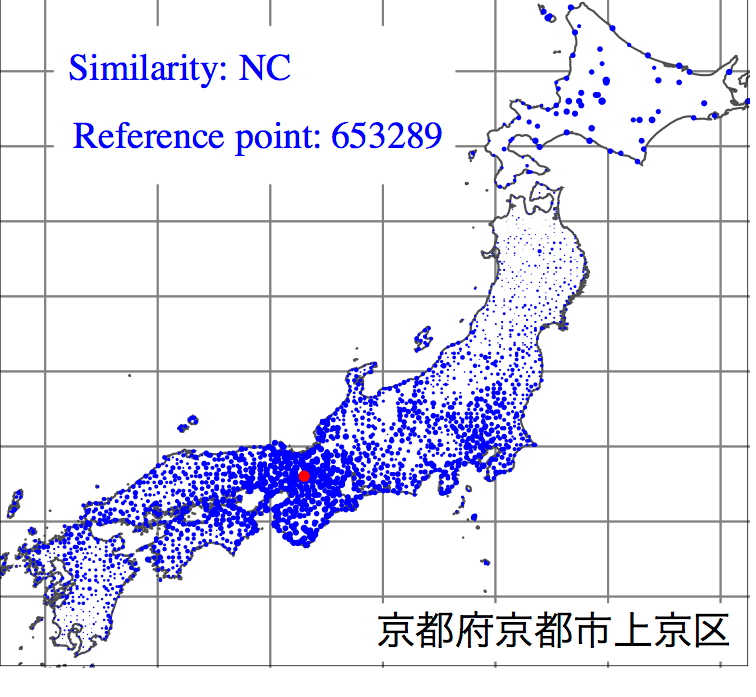
\includegraphics[width=0.32\textwidth]{illustrations/kuma_fig20-5}
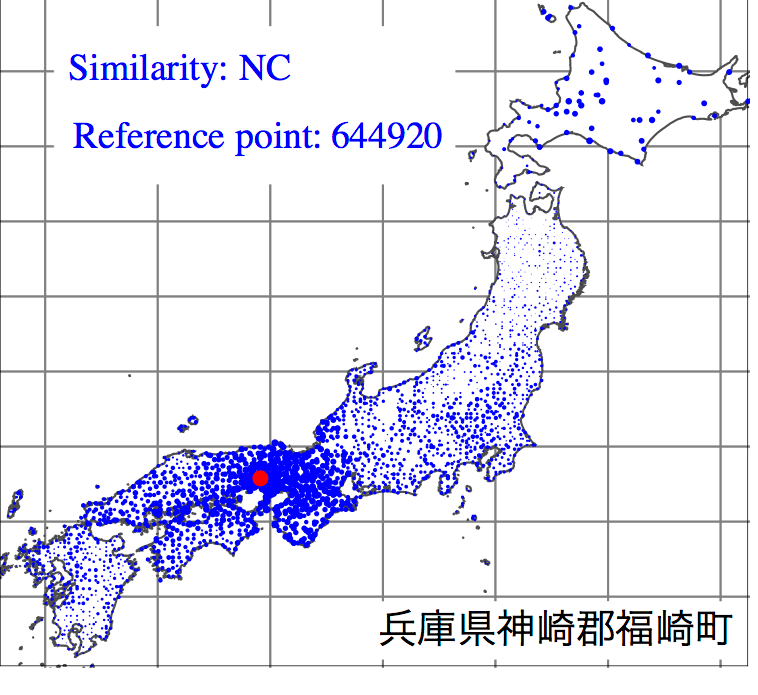
\includegraphics[width=0.32\textwidth]{illustrations/kuma_fig20-6}
\caption{Some example maps of geographical distributions of the degrees of similarity.}          
\label{fig:20}
\end{figure}

\figref{fig:21} presents similarity maps along the Nakasendo route. A total of 87 points along the Nakasendo route are selected by generating a buffer. Thus, we generated a series of similarity maps of points along a route (Nakasendo). The red line represents the Nakasendo route and the yellow points represent the selected localities. Playing the maps successively from Tokyo to Kyoto as animations facilitates observation of the changing patterns along the route. In \figref{fig:21}, some examples from the similarity maps (i.e. frames) are shown.

\figref{fig:22} displays an example of another kind of representation of linguistic similarity measured by NC among the localities. Delaunay triangulation—a computational geometrical method to generate a triangular network that connects adjacent points from randomly distributed points on a plane—is used as an approximation to represent continuity among survey points on the geographical space in a formal manner. A network of the points made by Delaunay triangulation is termed as a Delaunay net. We assign a value of NC (number of common linguistic features) to a line which connects two adjacent points of the Delaunay net to visualize the varying degrees of linguistic similarity among survey points distributed on a map. This representation is a network representation on a Delaunay net and is termed type n. Here, “n” represents NC \citep[2, 4]{kumagai_development_2013}. \figref{fig:23} presents another example; it provides a network representation of the degrees of similarities on a Delaunay net: type d (“d” denotes distance). The degree of linguistic similarity between adjacent localities is measured by the degree of similarity between the two NC distribution patterns of the localities. A distance matrix is calculated for this purpose. The degree of linguistic similarity between any two localities is measured by the Euclidean distance between the two NC distribution patterns \citep[2, 4]{kumagai_development_2013}, and is termed DC. The values of DC are categorized in the range of 100 in \figref{fig:23}. Due to space constraints, DC and these maps cannot be discussed in detail; however, clear patterns can be observed on these maps.

\begin{figure}
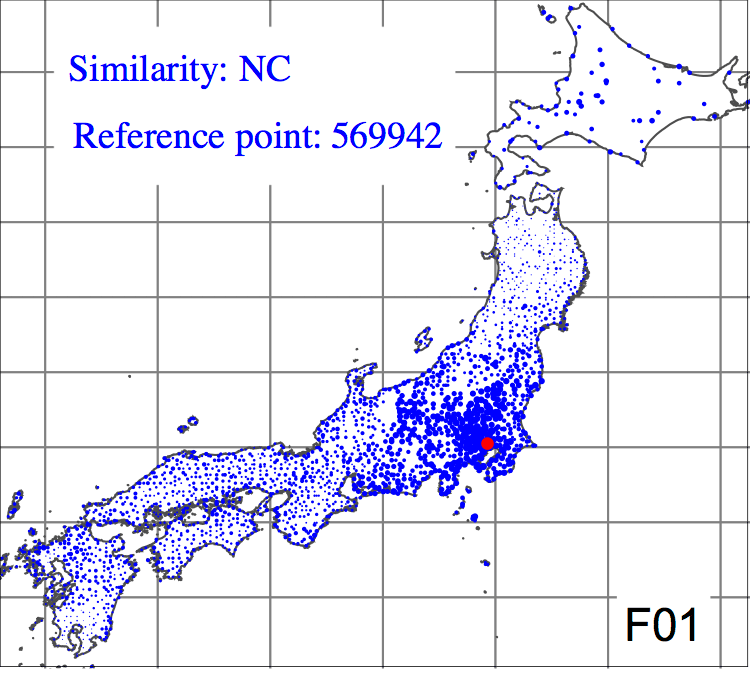
\includegraphics[width=0.32\textwidth]{illustrations/kuma_fig21-F01}
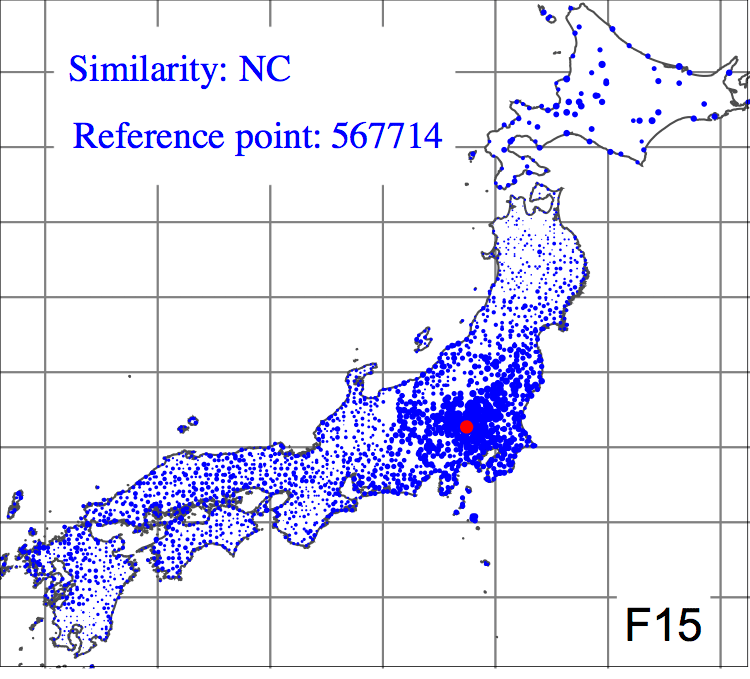
\includegraphics[width=0.32\textwidth]{illustrations/kuma_fig21-F15}
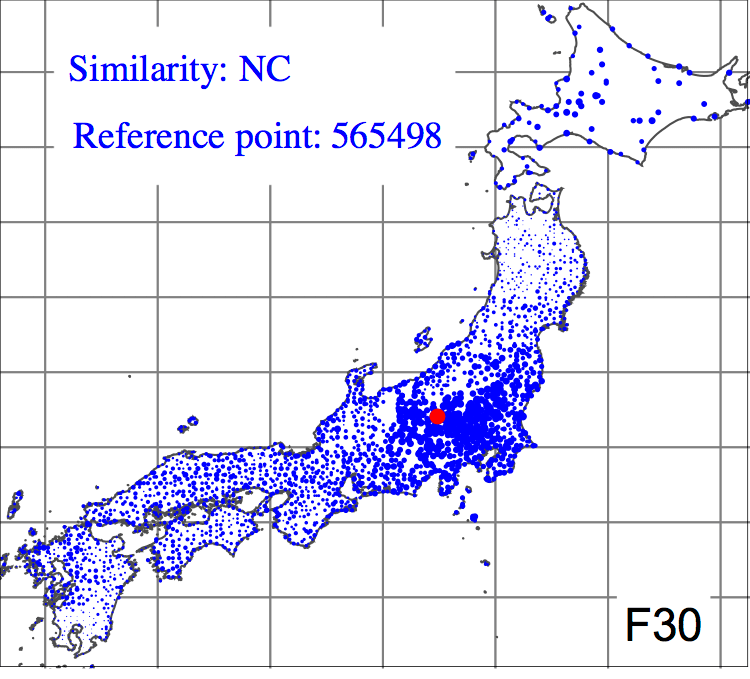
\includegraphics[width=0.32\textwidth]{illustrations/kuma_fig21-F30}
\\
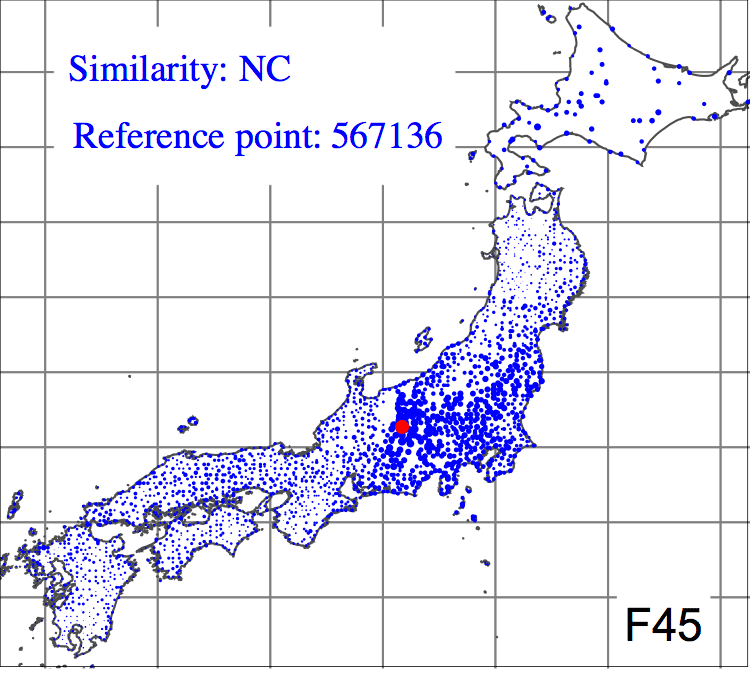
\includegraphics[width=0.32\textwidth]{illustrations/kuma_fig21-F45}
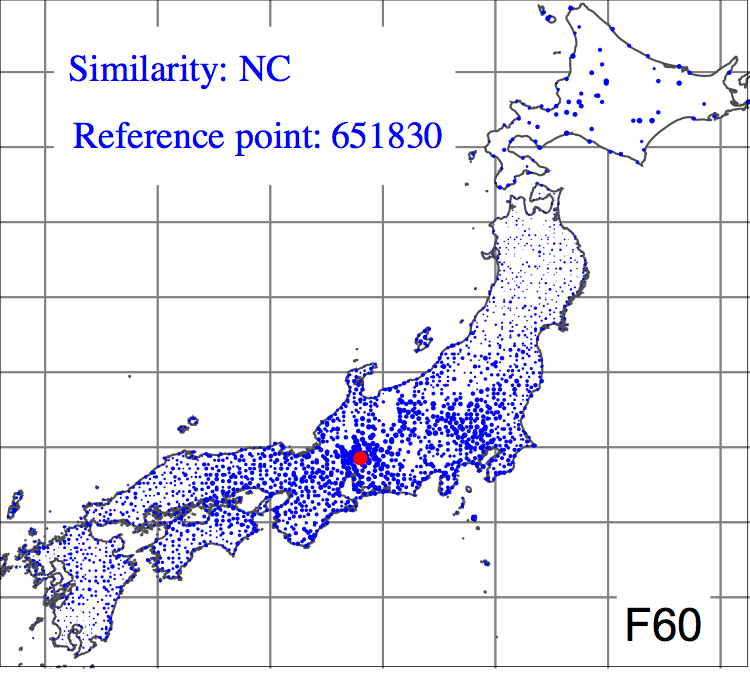
\includegraphics[width=0.32\textwidth]{illustrations/kuma_fig21-F60}
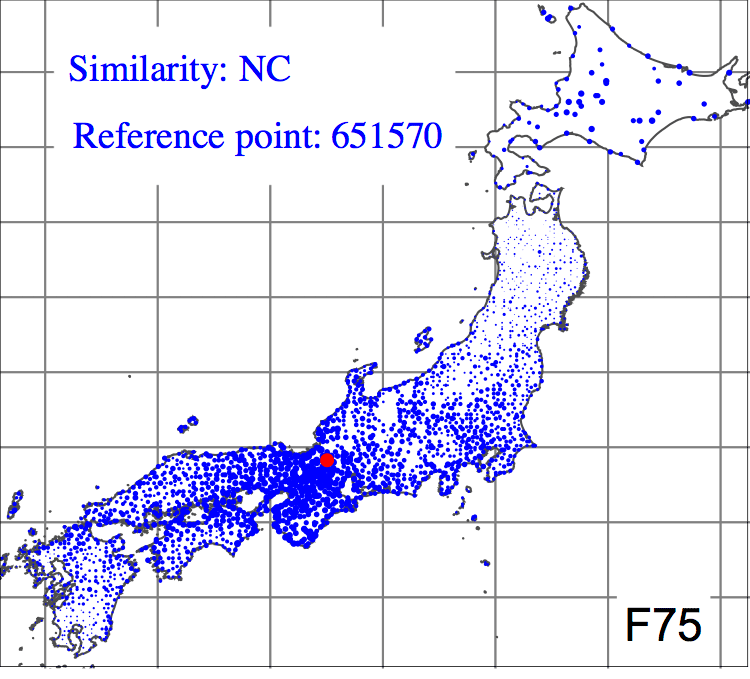
\includegraphics[width=0.32\textwidth]{illustrations/kuma_fig21-F75}
\\
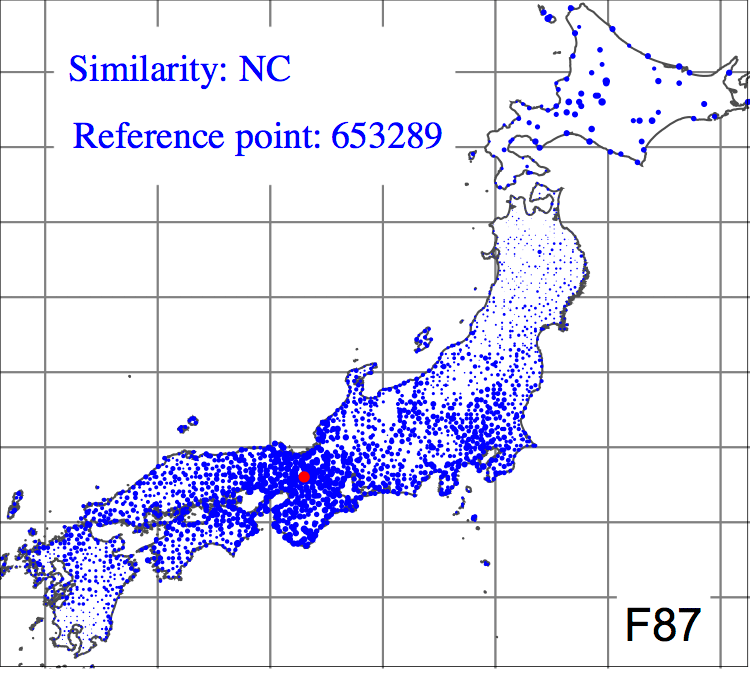
\includegraphics[width=0.32\textwidth]{illustrations/kuma_fig21-F87}
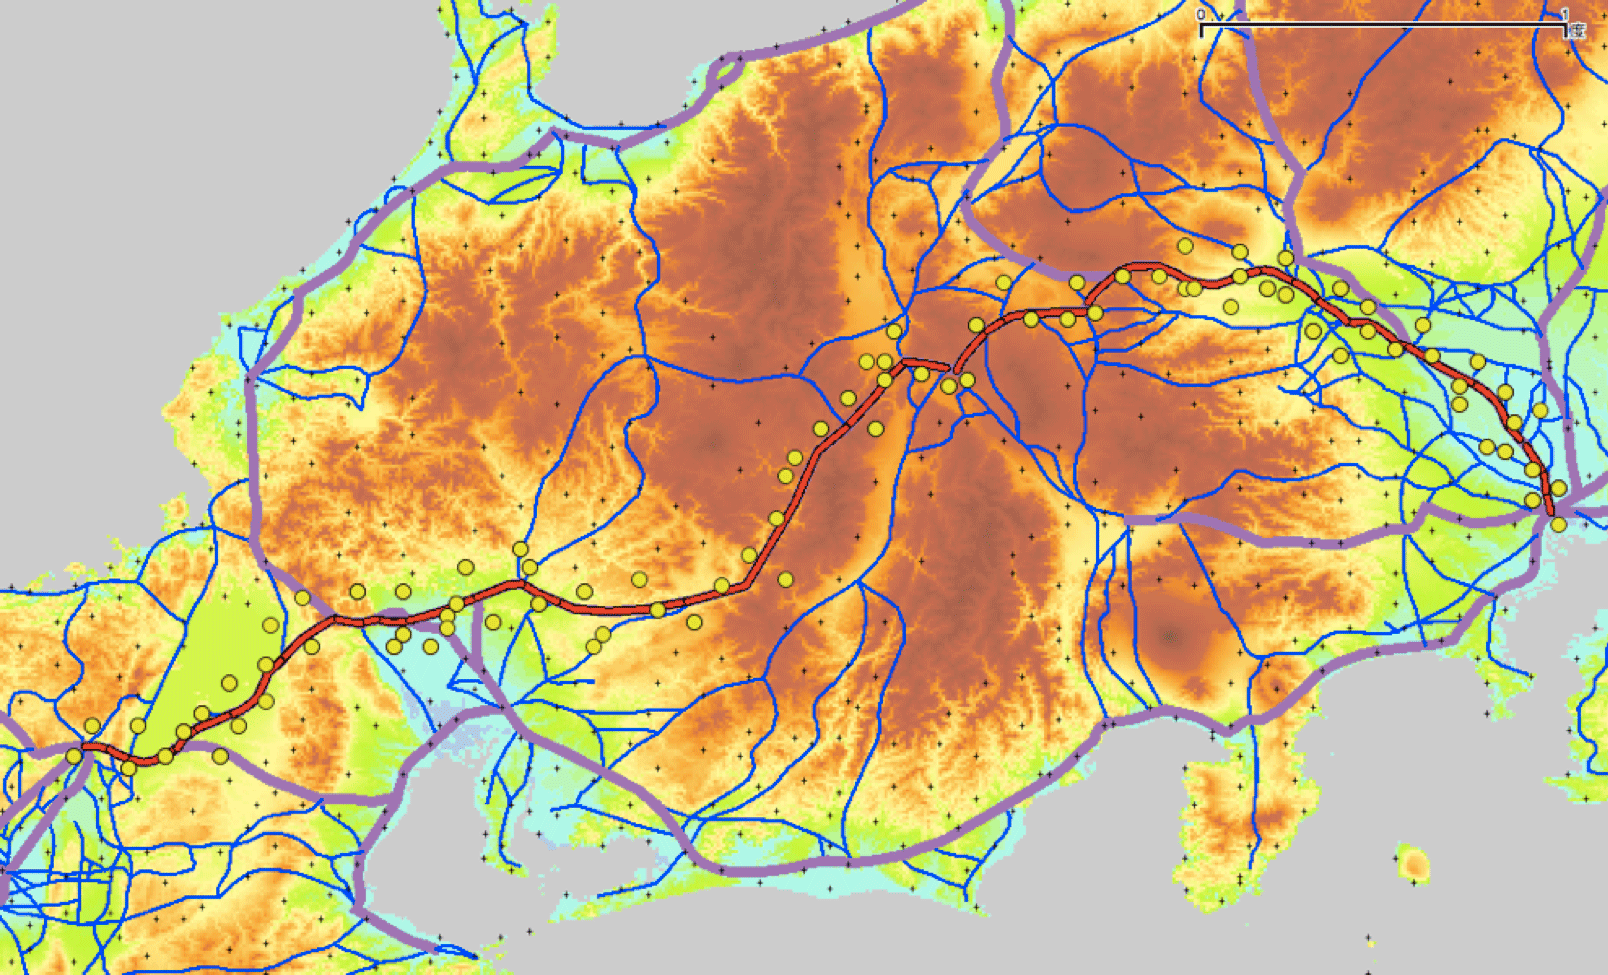
\includegraphics[width=0.66\textwidth]{illustrations/kuma_fig21-Points}
\caption{Some examples of similarity maps (frames of the animation) along the Nakasendo route. The number following F is a frame number. F01: Tokyo, F87: Kyoto. Bottom right: The 87 localities selected by buffer along the Nakasendo route (red line: Nakasendo; yellow points: selected localities).}          
\label{fig:21}
\end{figure}

\begin{figure}
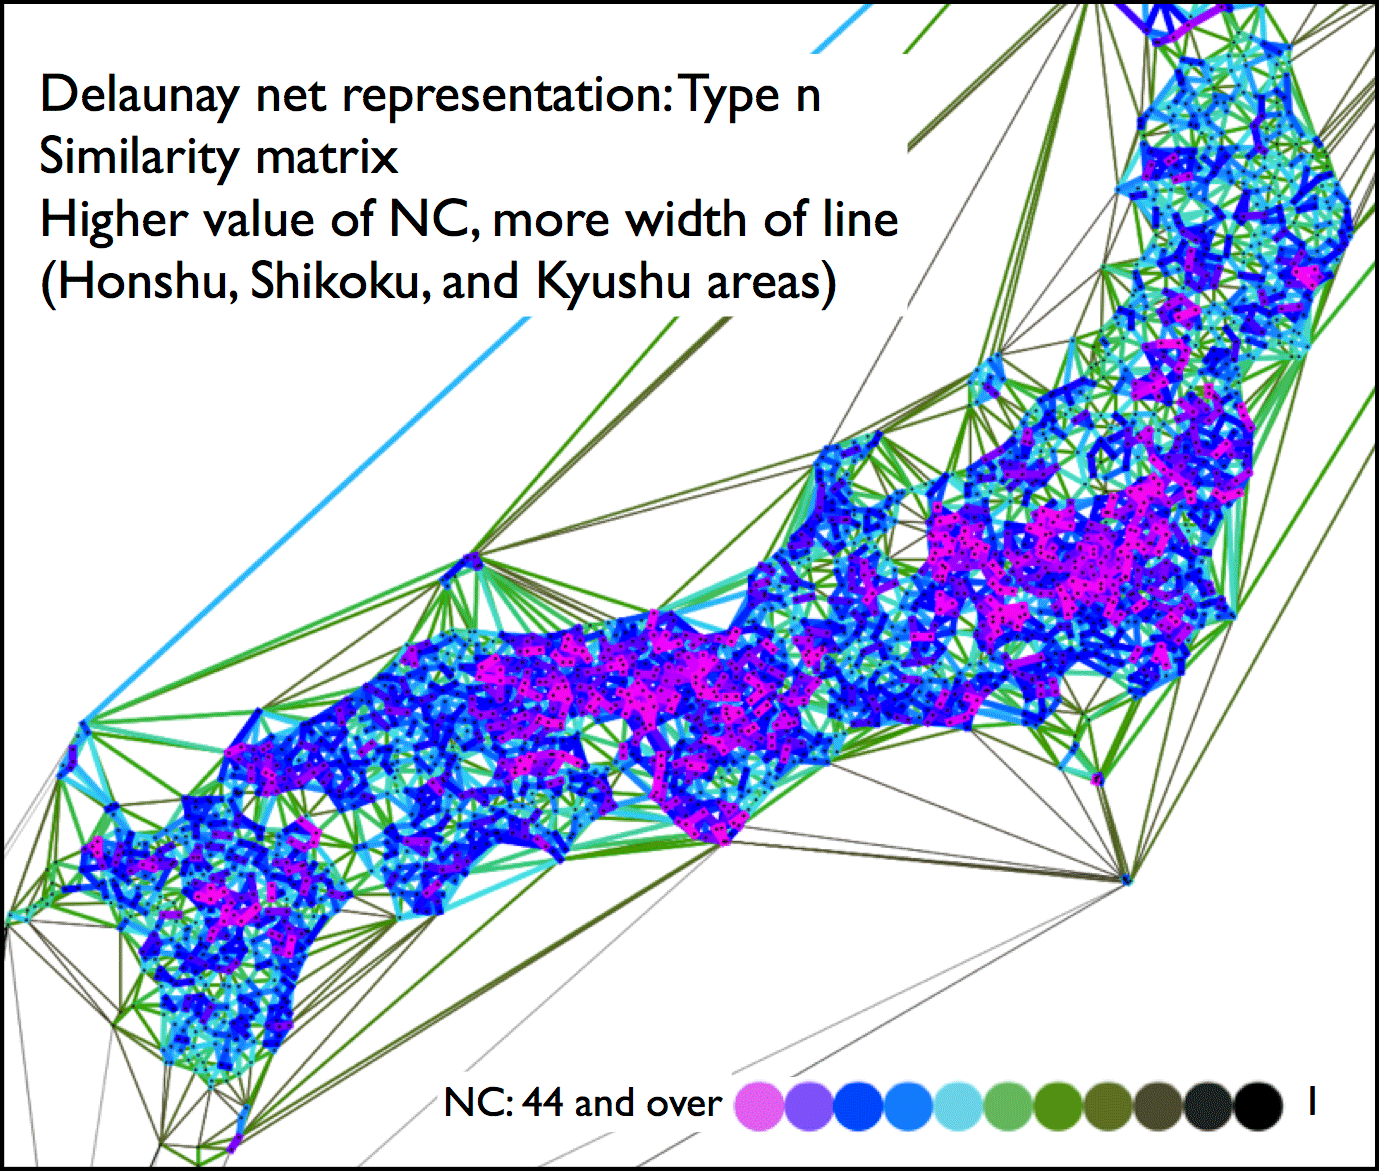
\includegraphics[width=0.8\textwidth]{illustrations/kuma_fig22}
\caption{Network representation of degrees of similarity on Delaunay net: Type n.}
\label{fig:22}
\end{figure}

\begin{figure}
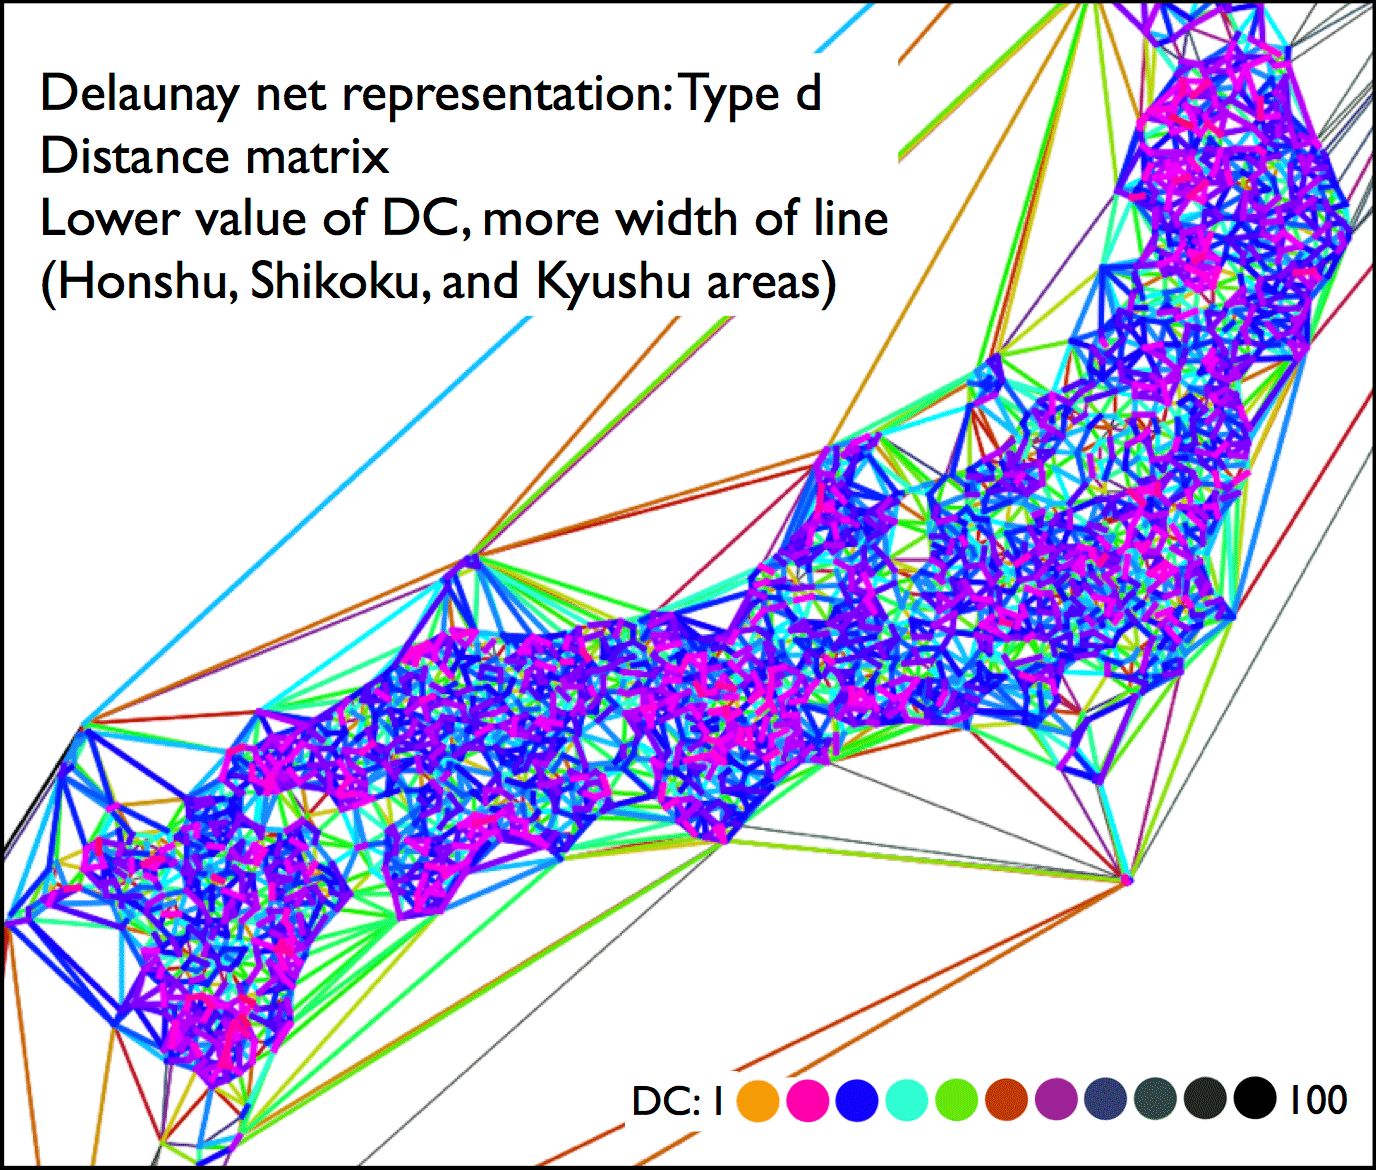
\includegraphics[width=0.8\textwidth]{illustrations/kuma_fig23}
\caption{Network representation of degrees of similarity on Delaunay net: Type d.}
\label{fig:23}
\end{figure}          

\begin{figure}
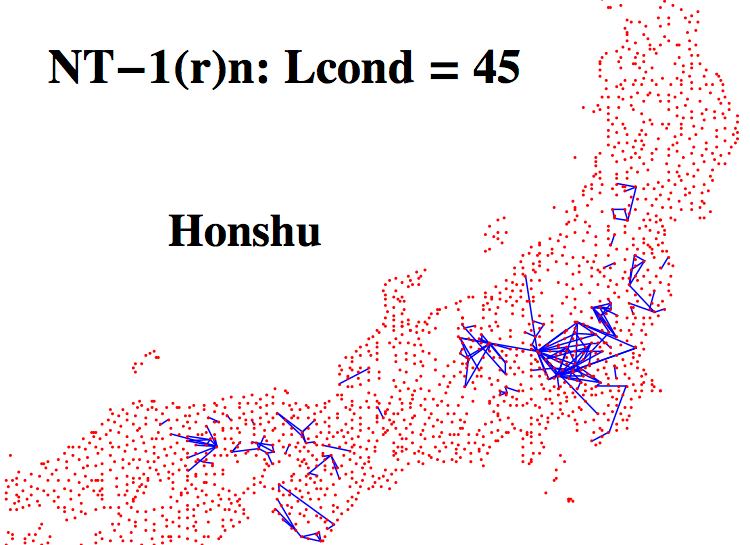
\includegraphics[width=0.3\textwidth]{illustrations/kuma_fig24-1}
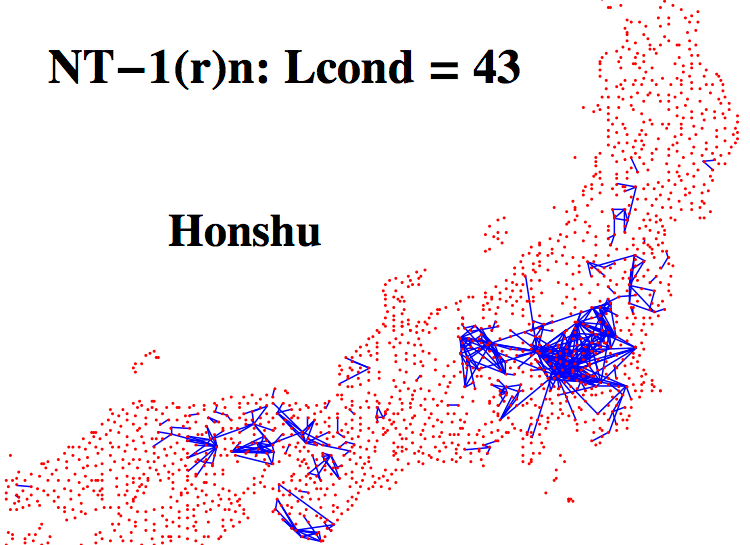
\includegraphics[width=0.3\textwidth]{illustrations/kuma_fig24-2}
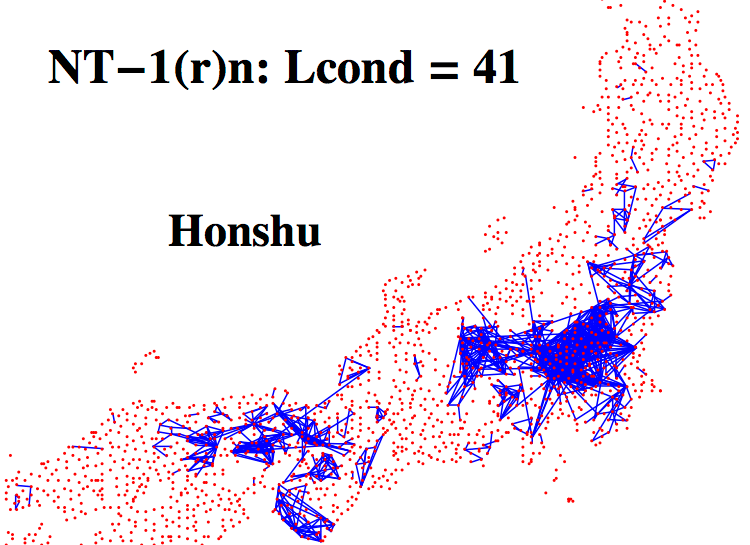
\includegraphics[width=0.3\textwidth]{illustrations/kuma_fig24-3}
\\
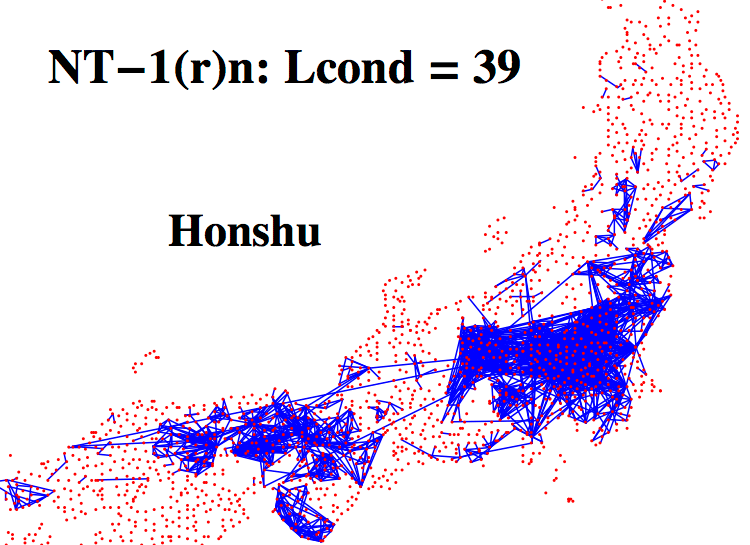
\includegraphics[width=0.3\textwidth]{illustrations/kuma_fig24-4}
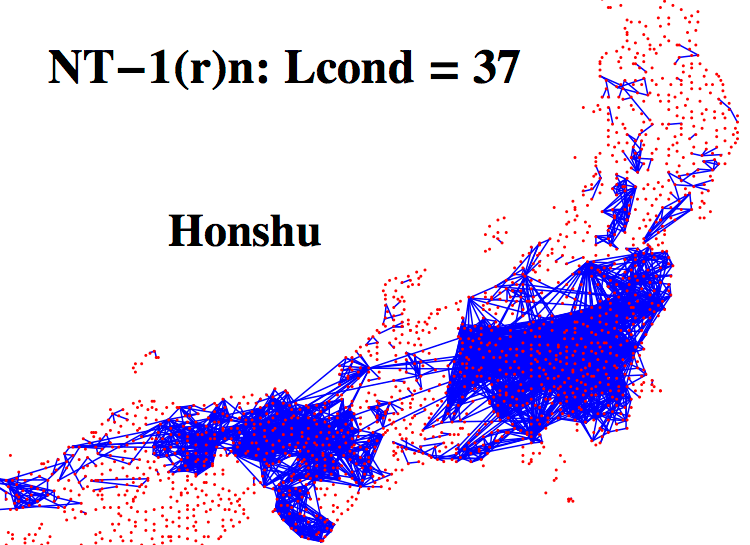
\includegraphics[width=0.3\textwidth]{illustrations/kuma_fig24-5}
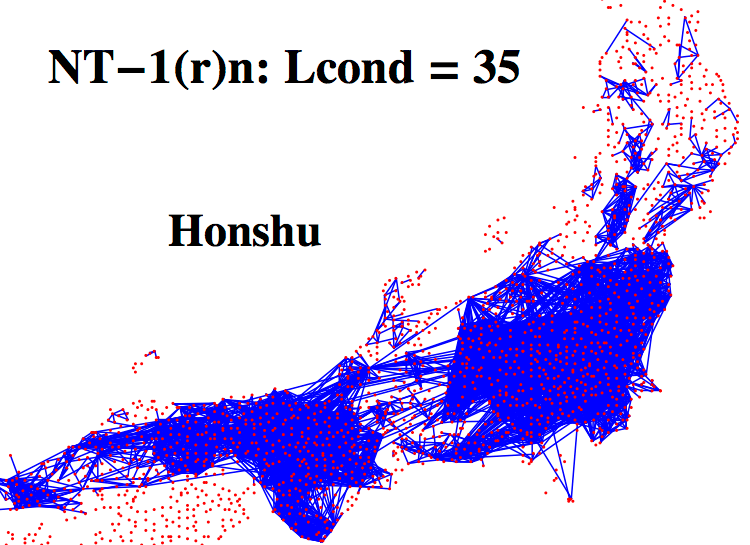
\includegraphics[width=0.3\textwidth]{illustrations/kuma_fig24-6}
\caption{Network representation of NT-1(r)n (Lcond = 45, 43, 41, 39, 37, 35).}
\label{fig:24}
\end{figure}

\figref{fig:24} shows the NT-1(r)n representation.\footnote{ In the Methods XV conference, this figure was represented as an animation with changing Lcond stepwise from 48 to 30. In \figref{fig:24}, some frames selected from the animation of NT-1(r)n are shown (LAJDB55).} NT-1(r)n is one of the series of methods we have developed to observe linguistic similarities among localities on a map \citep[2]{kumagai_development_2013}. In NT-1(r)n, any two localities that show similarities more than the threshold condition (Lcond) are connected by a line. The red points denote the localities. The measure of similarity used is NC. Any two localities that satisfy the threshold condition (NC \textsf{${\geqq}$ }Lcond) are connected by a line. In \figref{fig:24}, only the lines that connect localities inside the Honshu area are displayed to allow focus on observations inside this area. On changing the Lcond from 45 to 30, we can observe how the similar localities are distributed and how the clusters of similar localities grow. \figref{fig:25} displays a superimposition\footnote{By overlaying two types of representation, we can simultaneously observe the distribution of similarities along the continuity and on the entire map (which is not restricted to neighbors). In transitional zones and homogeneous zones, Nt-1(r) shows the different network structures. By overlaying the two kinds of representation, we can distinguish two types of distribution patterns of similarities, which cannot be distinguished by the representation of the Delaunay net \citep[7]{kumagai_development_2013}.} of the network representation NT-1(r)n on the Delaunay net type 2\footnote{ In the type 2 representation of the Delaunay net, a higher NC value corresponds with a lesser line width.} representation \citep[6--7]{kumagai_development_2013}. All figures in this section exhibited clear patterns and structures. 

It will be interesting to compare these patterns and structures with one another and with extra-linguistic features, such as road networks, to examine the relations among them. The previous observations made on the standard forms must be studied in relation to these observations.

\begin{figure}
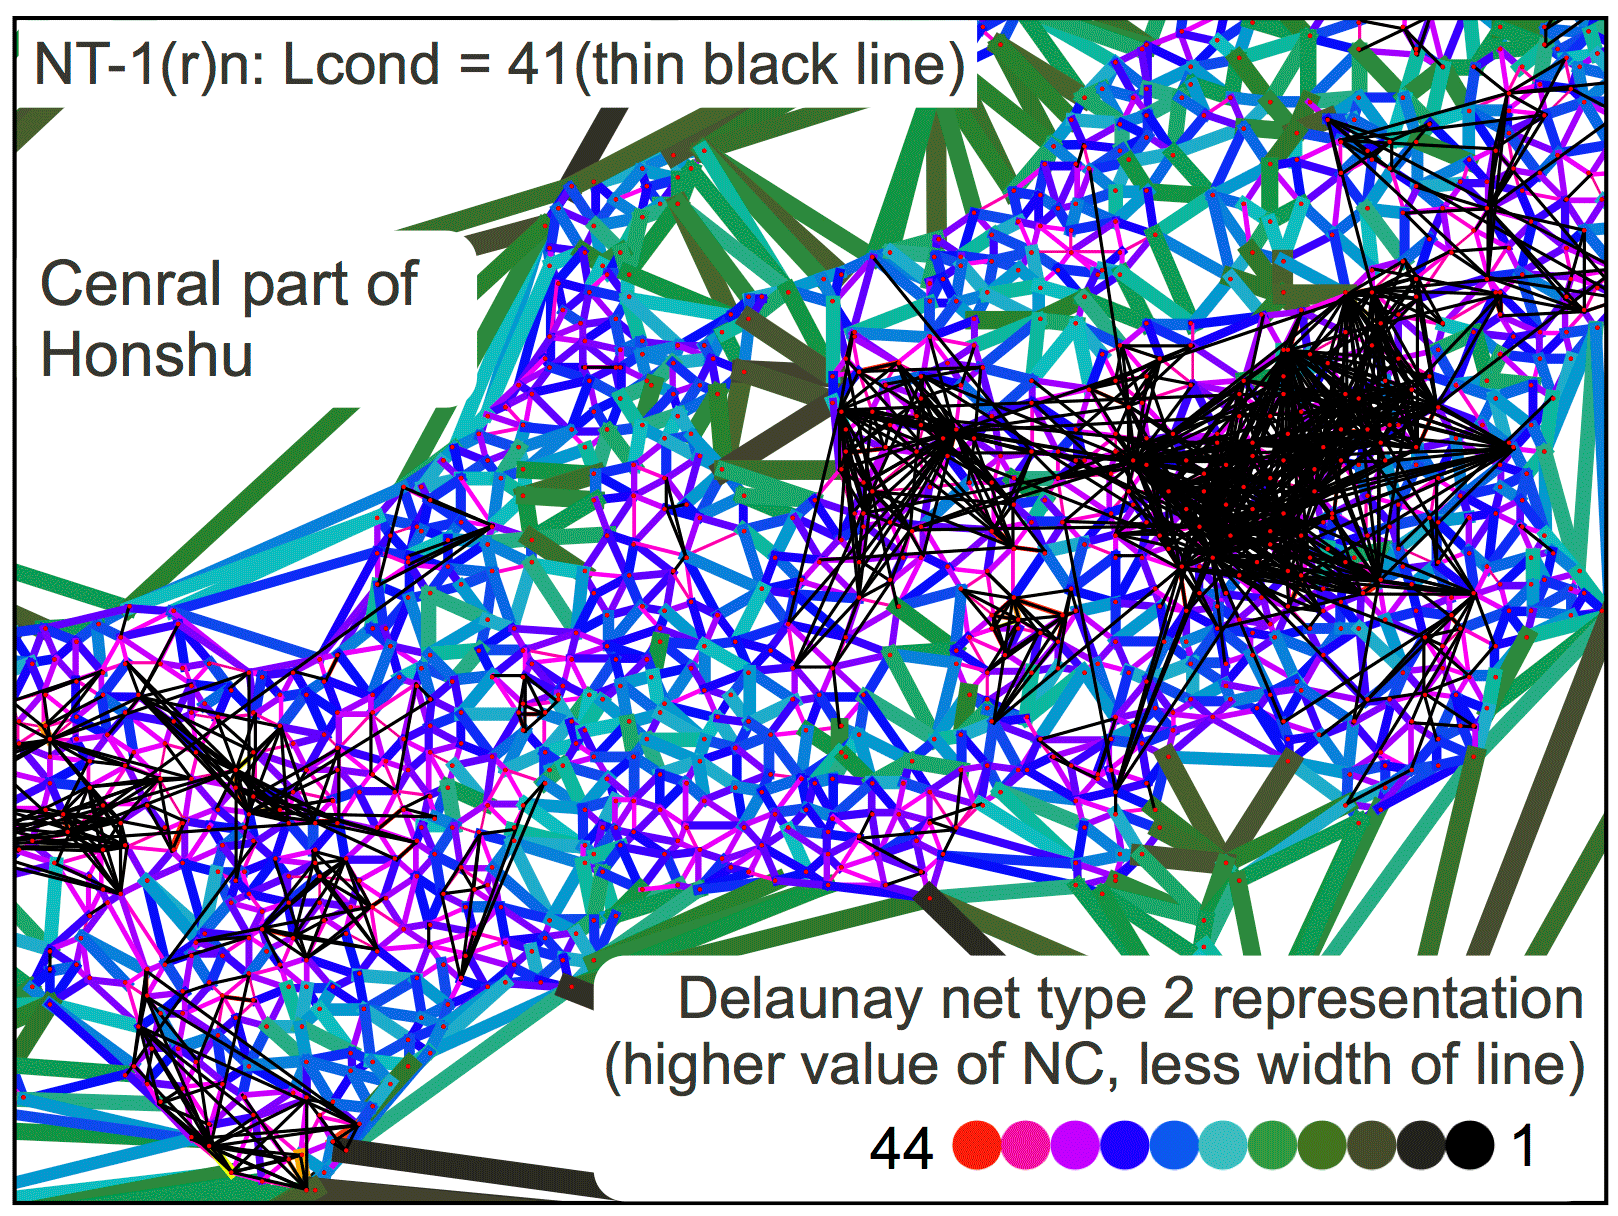
\includegraphics[width=0.8\textwidth]{illustrations/kuma_fig25}
\caption{Network representation NT-1(r)n on Delaunay net of type 2 representation.}
\label{fig:25}
\end{figure}  

\begin{figure}
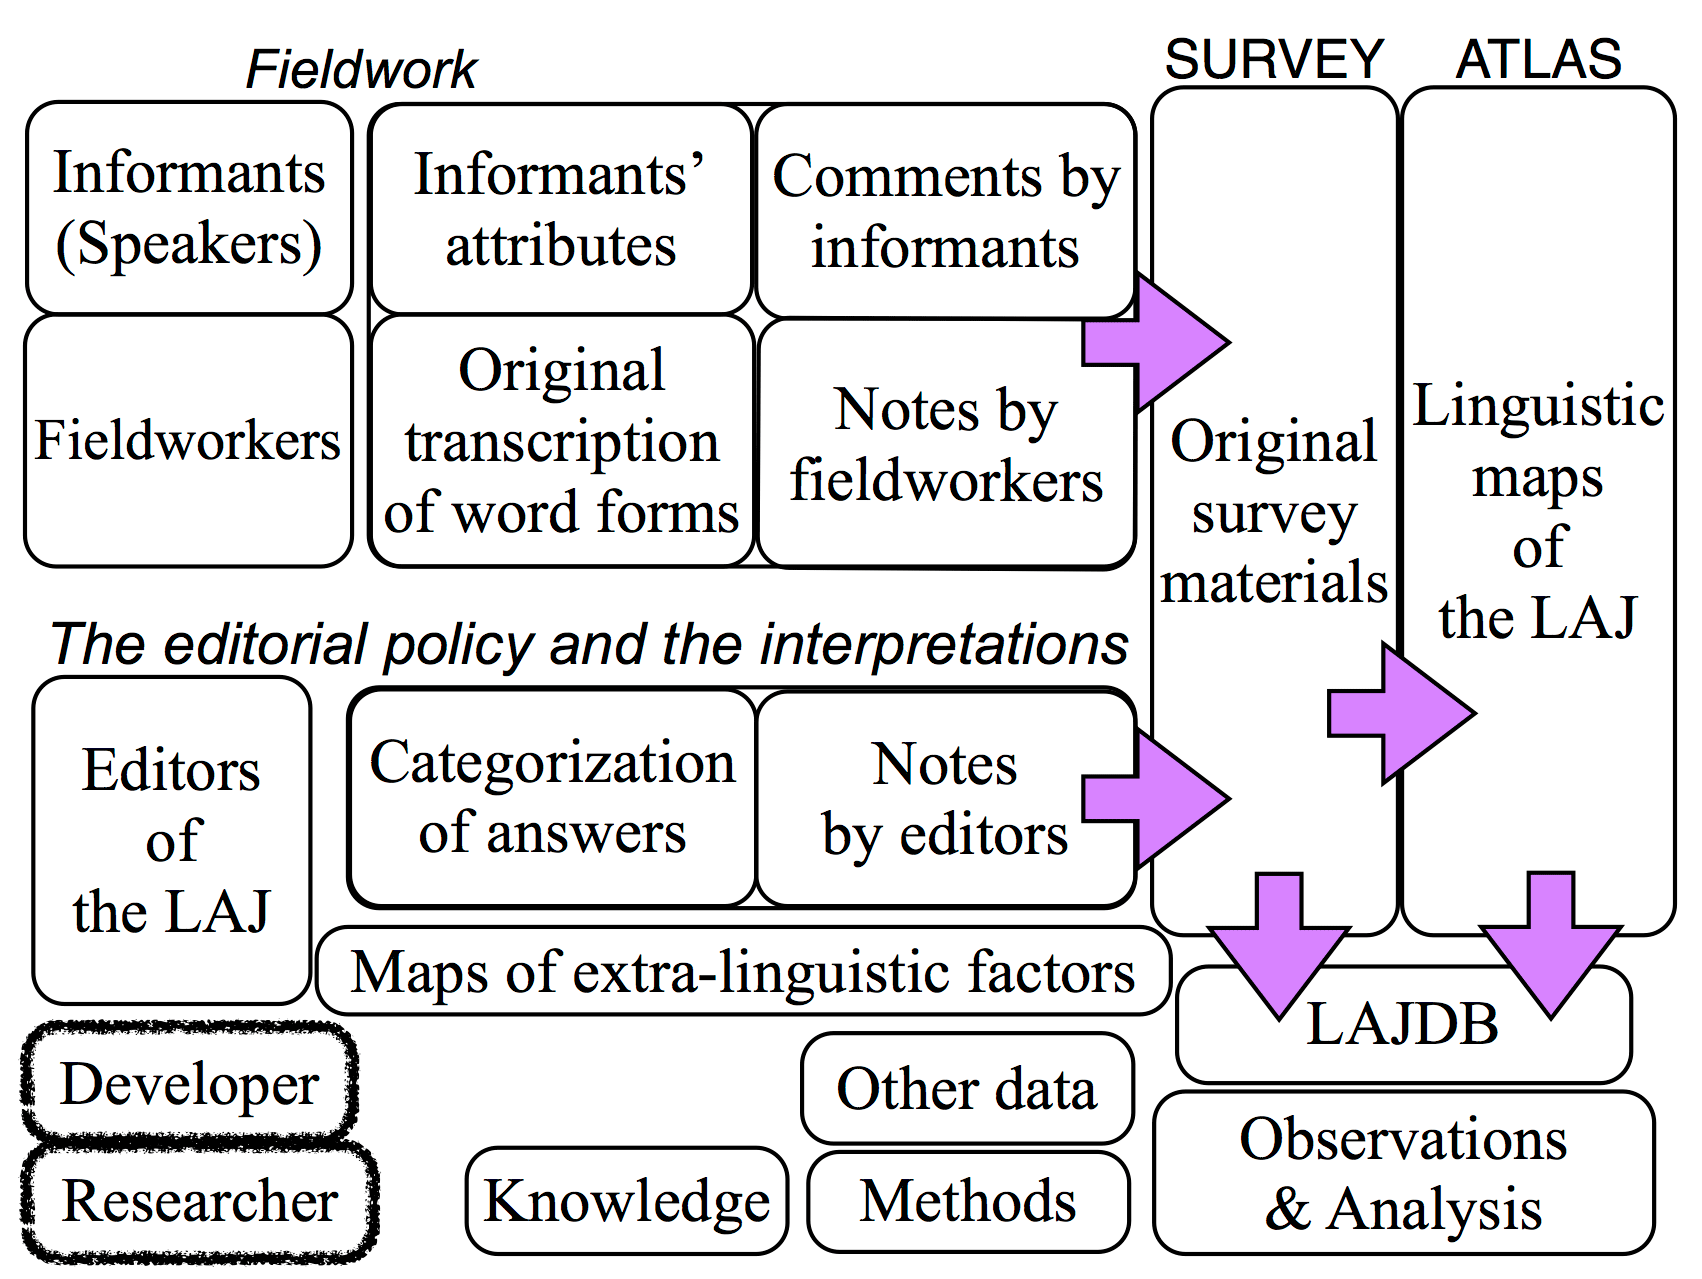
\includegraphics[width=0.8\textwidth]{illustrations/kuma_fig26}
\caption{Factors related to the development and utilization of the LAJDB.}
\label{fig:26}
\end{figure}  

\section{Conclusion}
We have been developing the LAJDB to preserve the original survey materials and advance the utilization of the LAJ. With 2400 localities, LAJDB data facilitates detailed observations of nationwide distributions, which are not possible with the prefecture-unit calculations in the LAJ. In linguistic maps, geographical distribution patterns of each word are usually recognized as distribution areas, that is, planar regions. However, the distributions recognized as planar regions are formed through contact between localities, such as transportation and intercommunication, which refers to contact between individuals (i.e., speakers). By accumulating items for 2400 localities, we will be able to observe the networks responsible for the formation of regions and the phenomena occurring in such networks. Further, we are developing methods for analyzing the geographical distribution data aimed at extracting latent information and finding hidden structure in a manner appropriate to the nature of the data, which will facilitate visualization of the dynamics, flows, and trends of dialectal distribution and understanding of the distribution pattern of dialects in relation to the dynamics of language change (\citealt{sibata_s&k_1993,kumagai_nihon_2013,kumagai_development_2013}, etc.). The researchers who conducted the LAJ survey designed many features and devices; however, these tools have not been sufficiently utilized. This shortcoming might partly result from the lack of computerized data, computers, and many other tools which are available today. 

\figref{fig:26} illustrates the factors that play an important role in the development and utilization of the LAJDB. All factors relate to developing the LAJDB and advancing the analysis of the geographical distribution of dialects. The digitized data of the LAJ and related information as well as the new methods and perspectives will contribute to advancing the analysis of the geographical distribution of dialects. The LAJDB\footnote{The LAJDB website is under development (\url{http://www.lajdb.org}). This website is currently a work-in-progress, and the LAJDB is only partially open. The site will be updated in accordance with LAJDB progress.} is expected to be a good tool for utilizing the LAJ and to contribute to advancing the study of the geographical distribution of dialects. 

\section*{Abbreviations}
\setlength{\parindent}{0pt}\begin{tabbing}
LAJDB55\hspace{.75em} \= a subset of LAJDB\kill
LAJ	\> Linguistic Atlas of Japan\\
LAJDB \>	Linguistic Atlas of Japan Database\\
LAJDB42	\> a subset of LAJDB55\\
LAJDB55 \> a subset of LAJDB\\
NLRI	\> National Language Research Institute\\
NINJAL	\> National Institute for Japanese Language and Linguistics\\
NORM	\> non-mobile, older, rural males\\
GDF	\> geographical distributions of frequency\\
NC \> number of common linguistic features (number of common word\\
	\> forms)\\
GIS	\> geographic information system\\
NT-1(r)n	\> a method of network representation of linguistic similarities\\
Lcond	\> level conditioned (threshold condition)
\end{tabbing}\setlength{\parindent}{10pt}

\section*{Acknowledgements}
The Linguistic Atlas of Japan Database (LAJDB) was supported by a Grant-in-Aid for Publication of Scientific Research Results (database) in 2001, 2002, 2003, 2004, 2005, and 2008 (Project Leader: Yasuo Kumagai). This paper includes some outcomes of the collaborative research projects “Analyzing large-scale dialectal survey data from multiple perspectives” (2009–2012, Project Leader: Yasuo Kumagai), “General Research for the Study and Conservation of Endangered Dialects in Japan” (2013–, Project Leader: Nobuko Kibe) at the National Institute for Japanese Language and Linguistics, and “Development of quantitative methods of analyzing large-scale dialectal distribution data” (Grants-in-aid for scientific research (c), JSPS KAKENHI Grant Number 26370555, 2014–, Project Leader: Yasuo Kumagai). I thank the anonymous reviewers and the editors for their valuable comments and suggestions.

\printbibliography[heading=subbibliography,notkeyword=this]
\end{document}